% !TEX root = saveliev_physics_general_course_1.tex
%!TEX TS-program = pdflatex
%!TEX encoding = UTF-8 Unicode


\chapter{ĐỘNG HỌC}\label{chap:1}

\section{Chuyển động cơ học}\label{sec:1_1}

Chuyển động cơ học có mặt trong sự chuyển dịch của các vật hoặc của các phần của vật với nhau là dạng chuyển động đơn giản nhất của vật chất. Chúng ta thường xuyên quan sát được sự dịch chuyển của các vật trong đời sống hàng ngày. Vì thế mà các khái niệm cơ học là rất cụ thể. Điều này giải thích tại sao trong tất cả các khoa học tự nhiên thì cơ học phát triển rộng rãi trước các khoa học khác.

Tập hợp các vật được tách riêng ra để nghiên cứu được gọi là một \textbf{hệ cơ học}. Cần phải đưa các vật nào vào hệ là tùy thuộc vào tính chất của các bài toán phải giải. Đôi khi hệ có thể gồm một vật duy nhất.

Trên đây đã chỉ ra rằng trong cơ học sự thay đổi vị trí tương hỗ của các vật được gọi là sự chuyển động. Nếu tưởng tượng một vật cô lập tách biệt nằm trong không gian, trong đó không có các vật khác thì ta không thể nói về chuyển động của nó, vì chẳng có cái gì để vật này có thể thay đổi vị trí của mình đối với cái đó. Từ đó suy ra rằng nếu ta tập trung nghiên cứu chuyển động của một vật nào đó thì nhất thiết cần phải chỉ ra chuyển động này xảy ra đối với các vật nào khác.

Chuyển động xảy ra cả trong không gian và cả trong thời gian (không gian và thời gian là các dạng không thể tách rời được của sự tồn tại của vật chất).Do đó để mô tả chuyển động cũng cần phải xác định thời gian. Điều này được thực hiện nhờ đồng hồ.

Tập hợp các vật không chuyển động đối với nhau mà người ta khảo sát sự chuyển động đối với chúng và các đồng hồ tính thời gian tạo thành một \textbf{hệ quy chiếu}.

Chuyển động của cùng một vật đối với các hệ quy chiếu khác nhau có thể có tính chất khác nhau. Để làm ví dụ ta hãy tưởng thượng một đoàn tàu đang tăng vận tốc. Giả thử rằng một hành khách đi dọc theo hành lang của một toa tàu với vận tốc không đổi. Khi đó chuyển động của hành khách đối với toa tàu là chuyển động đều, còn đối với mặt đất là chuyển động có gia tốc.

Mô tả chuyển động của vật có nghĩa là chỉ ra vị trí trong không gian và vận tốc của vật tại mỗi thời điểm. Muốn vậy khi cho trạng thái của một hệ cơ, cần phải chỉ ra vị trí và vận tốc của tất cả các vật tạo thành hệ. Bài toán điển hình của cơ học là nếu biết trạng thái của một hệ tại thời điểm ban đầu ${t_o}$ nào đó, và cả những định luật chi phối sự chuyển động thì xác định được trạng thái của hệ tại mọi thời điểm $t$ tiếp theo.

Ta hãy chú ý rằng không có một bài toán vật lý nào có thể được giải một cách chính xác tuyệt đối. Người ta luôn luôn thu được lời giải gần đúng. Mức độ gần đúng được xác định bằng tính chất của bài toán một cách gần đúng, người ta bỏ qua một số sự kiện mà trong trường hợp đã cho là không quan trọng. Chẳng hạn như, thường có thể bỏ qua các kích thước của vật mà ta nghiên cứu chuyển động của nó. Chẳng hạn, khi nghiên cứu chuyển động của Trái đất xung quanh Mặt trời thì hoàn toàn có thể bỏ qua các kích thước của Trái đất. Do đó sự mô tả chuyển động được đơn giản hóa một cách đáng kể, nghĩa là có thể xác định được vị trí của Trái đất trong không gian bằng một điểm.

Một vật mà trong những điều kiện của bài toán đã cho có thể bỏ qua các kích thước của nó được gọi là một \textbf{chất điểm}. Vấn đề là ở chỗ có thể coi một vật cụ thể đã cho như một chất điểm hay không, sẽ tùy thuộc không phải vào các kích thước của vật này mà vào các điều kiện của bài toán. Cùng một vật, trong những trường hợp này có thể coi là một chất điểm còn trong những trường hợp khác phải được coi như một vật lớn.


Khi nói về một vật nào đó như về một chất điểm, ta trừu tượng hóa các kích thước của nó. Một sự trừu tượng hóa thứ hai ta đã từng gặp trong cơ học - đó là vật rắn tuyệt đối. Trong thiên nhiên không có các vật hoàn toàn không biến dạng. Mỗi vật dưới tác dụng của các lực đặt lên nó, sẽ bị biến dạng hoặc nhiều hoặc ít, tức là biến đổi hình dạng và các kích thước của mình. Tuy nhiên trong nhiều trường hợp có thể bỏ qua các sự biến dạng của các vật khi nghiên cứu chuyển động của chúng. Nếu điều này xảy ra thì người ta gọi vật là vật rắn tuyển đối. Như vậy, một vật mà trong những điều kiện đã cho của bài toán có thể bỏ qua các biến dạng được gọi là \textbf{vật rắn tuyệt đối}.

Có thể phân tích mỗi chuyển động của vật rắn thành hai dạng chuyển động cơ bản là \textbf{chuyển động tịnh tiến} và \textbf{chuyển động quay}.

Chuyển động tịnh tiến - đó là chuyển động mà một đường thẳng bất kỳ gắn với vật chuyển động sẽ vẫn song song với chính nó (\fig{1_1}).

Trong chuyển động quay, mọi điểm của vật được chuyển động theo các đường tròn có tâm nằm trên cùng một đường thẳng gọi là \textbf{trục quay} (\fig{1_2}). Trục quay có thể nằm ở ngoài vật (xem \fig{1_2}b).

\begin{figure}[!htb]
	\begin{minipage}[t]{0.5\linewidth}
		\begin{center}
			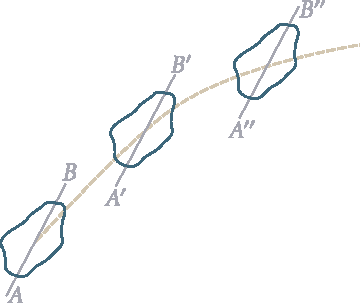
\includegraphics[scale=0.95]{figures/ch_01/fig_1_1.pdf}
			\caption[]{}
			\label{fig:1_1}
		\end{center}
	\end{minipage}
	\hfill{ }%\hspace{-0.1cm}
	\begin{minipage}[t]{0.5\linewidth}
		\begin{center}
			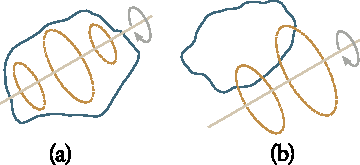
\includegraphics[scale=0.95]{figures/ch_01/fig_1_2.pdf}
			\caption[]{}
			\label{fig:1_2}
		\end{center}
	\end{minipage}
\end{figure}

Vì khi nói về một vật nào đó như về một chất điểm ta lãng quên quảng tính của nó nên khái niệm chuyển động quay quanh một trục xuyên qua nó là không áp dụng được cho vật đó.

Để có được khả năng mô tả chuyển động một cách định lượng, cần phải gắn với các vật tạo thành hệ quy chiếu một hệ tọa độ nào đó, chẳng hạn hệ tọa độ Descartes. Khi đó có thể sách định vị trí của chất điểm nếu cho ba số $x$, $y$, $z$ là các tọa độ Descartes của điểm này. Có thể thực hiện một hệ tọa độ, bằng việc chọn một mạng vuông góc gồm những thanh hoặc những thước tỷ lệ như nhau (\fig{1_3}). Tại các nút mạng này cần phải đặt các đồng hồ đồng bộ với nhau và giống hệt nhau. Vị trí của chất điểm và thời điểm ứng với nó được ghi theo các thang tỷ lệ và đồng hồ ở gần chất điểm nhất.

\begin{figure}[!htb]
	\begin{center}
		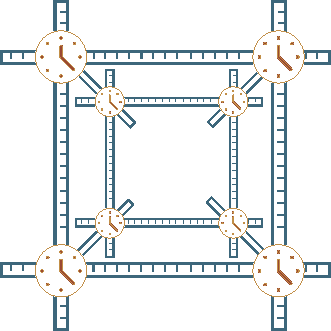
\includegraphics[scale=0.95]{figures/ch_01/fig_1_3.pdf}
		\caption[]{}
		\label{fig:1_3}
	\end{center}
\end{figure}

Đề cập tới một chất điểm, sẽ đơn giản hơn là đề cập tới một vật có kích thước dài. Do đó bước đầu chúng ta sẽ nghiên cứu cơ học của chất điểm, và sau đó ta sẽ chuyển qua cơ học của vật rắn. Ta bắt đầu trình bày từ động học, sau đó ta sẽ đi vào động lực học. Ta nhớ rằng \textbf{động học} nghiên cứu sự chuyển động của các vật mà không chú ý tới các nguyên nhân gây ra chuyển động này. \textbf{Động lực học} nghiên cứu chuyển động của các vật liên hệ với các nguyên nhân (với các tương tác giữa các vật) gây ra một tính chất nào đó của chuyển động.

\section{Một số kiến thức về vector}\label{sec:1_2}

\textbf{Định nghĩa vector.} Nguời ta gọi vector là một đại lượng được đặc trưng bằng trị số và hướng và ngoài ra có thể cộng theo quy tắc hình bình hành\footnote{Theo một định nghĩa chặt chẽ hơn, người ta gọi vector là một tập hợp ba đại lượng biến đổi theo một quy luật xác định khi quay các trục tọa độ.}. Yêu cầu sau cùng này là rất quan trọng. Có thể nêu ra các đại lượng mà chúng được đặc trưng bằng trị số và hướng, tuy nhiên được cộng khắc hẳn với các vector. Để làm ví dụ, ta hãy đưa ra sự quay của một vật quanh một trục nào đó một góc hữu hạn $\varphi$. Có thể biểu diễn sự quay như thế dưới dạng một đoạn thẳng có độ dài là $\varphi$, hướng theo trục mà phép quay được thực hiện xung quanh nó, về phía liên kết với chiều quay bằng quy tắc cái đinh ốc thuận. Trên \fig{1_4} ở dãy trên người ta đưa ra hai phép quay liên tiếp nhau của một quả cầu theo những góc $\pi/2$ được biểu diễn bằng các đoạn thẳng $\varphi_1$ và $\varphi_2$. Phép quay thứ nhất được thực hiện xung quanh trục $1$---$1$, dịch chuyển điểm  $A$ của quả cầu sang vị trí $A'$, được thực hiện xung quanh trục $2$---$2$, sang vị trí $A''$. Có thể đạt được cùng một kết quả như thế (tức là dịch chuyển điểm $A$ sang vị trí $A''$) bằng cách quay quả cầu xung quanh trục $3$---$3$ (xem dãy dưới ở \fig{1_4}) một góc $\pi$. Do đó cần phải coi phép quay đó như tổng của các phép quay $\varphi_1$ và $\varphi_2$. Tuy nhiên không thể có được nó từ những đoạn thẳng $\varphi_1$ và $\varphi_2$, bằng cách cộng chúng theo qui tắc hình bình hành. Một phép cộng như thế cho một đoạn thẳng có độ dài $\pi/\sqrt{2}$ thay cho độ dài $\pi$ cần phải có. Phép quay một góc $\pi/\sqrt{2}$ dịch chuyển điểm $A$ tới điểm $A'''$. Từ đó suy ra rằng các phép quay những góc hữu hạn được biểu diễn bằng những đoạn thẳng có hướng đều không có các tính chất của các vector.

\begin{figure}[!htb]
	\begin{center}
		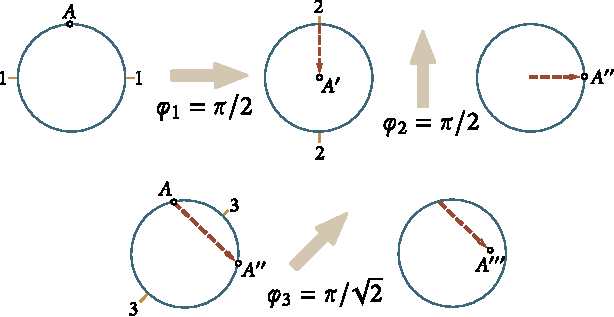
\includegraphics[scale=0.9]{figures/ch_01/fig_1_4.pdf}
		\caption[]{}
		\label{fig:1_4}
	\end{center}
\end{figure}

Trị số của vector được gọi là \textbf{module} của nó. Nói cách khác, module cho độ dài của vector. Module của vector là một vô hướng, do đó luôn luôn dương.

Trên các hình vẽ, các vector được biểu diễn dưới dạng các đoạn thẳng với mũi tên ở đầu. Độ dài của đoạn thẳng xác định module của vector trong tỷ lệ xích được thiết lập, còn mũi tên chỉ chiều của vector.

Người ta thường ký hiệu các vector bằng các chữ in đậm, chẳng hạn như $\vec{a}$, $\vec{b}$, $\vec{v}$ và $\vec{F}$. Cũng như thế nhưng in thường được dùng để ký hiệu module của vector $\vec{a}$\footnote{Trong khi viết, các vector được ký hiệu bằng các chữ với mũi tên ở trên chúng (chẳng hạn như $\oldvec{a}$). Trong trường hợp này, chính chữ đó mà không có mũi tên sẽ là module của vector.}. Đôi khi để ký hiệu module, đành phải dùng ký hiệu của vector đặt giữa hai vạch thẳng đứng: $|a|$ = module của vector $\vec{a}$. Cách ký hiệu như thế được sử dụng chẳng hạn cho module của tổng các vector $\vec{a}_1$ và $\vec{a}_2$:
\begin{equation}\label{eq:1_1}
	|\vec{a}_1 + \vec{a}_2| = \text{module của vector } (\vec{a}_1 + \vec{a}_2).
\end{equation}

\noindent
Trong trường hợp này ký hiệu $a_1+a_2$ có nghĩa là tổng các module của các vector số hạng, nói chung, không bằng module của tổng các vector (đẳng thức chỉ xảy ra trong trường hợp các vector có cùng hướng).

Các vector hướng dọc theo các đường thẳng song song cùng chiều hoặc ngược chiều nhau được gọi là các \textbf{vector đồng phương}. Các vector nằm trong các mặt phẳng song song được gọi là các \textbf{vector đồng phẳng}. Bằng sự dịch chuyển song song, các vector đồng phương có thể được đặt dọc theo cùng một đường thẳng, còn các vector đồng phẳng có thể được quy về một mặt phẳng.

Những vector đồng phương trùng nhau về module có cùng hướng được xem là bằng nhau\footnote{Lưu ý đến các \textbf{vector tự do}, nghĩa là các vector mà chúng có thể được đặt tại bất kỳ điểm nào trong không gian. Người ta cũng coi các \textbf{vector trượt} là các vector có gốc có thể được đặt tại bất kỳ điểm nào trên đường thẳng mà các vector được hướng dọc theo đó và các \textbf{vector buộc} nghĩa là các vector được đặt tại một điểm xác định. Hai dạng vector sau cùng này có thể được biểu thị qua các vector tự do: vì lý do này mà khái niệm vector tự do, thường được gọi đơn giản là vector, đã được đặt làm cơ sở cho phép tính vector.}

\textbf{Phép cộng và trừ các vector.} Để thuận tiện hơn, trong thực tế, khi cộng các vector người ta không vẽ hình bình hành. Như đã thấy trong \fig{1_5} người ta sẽ đạt được cùng một kết quả nếu đặt gốc của vector thứ hai trùng với ngọn của vector thứ nhất và sau đó vẽ vector tổng từ gốc của vector thứ nhất tới ngọn của vector thứ hai. Phương pháp như thế đặc biệt có lợi trong trường hợp khi phải cộng một số lượng vector lớn hơn hai (\fig{1_6}).

\begin{figure}[!htb]
	\begin{minipage}[t]{0.5\linewidth}
		\begin{center}
			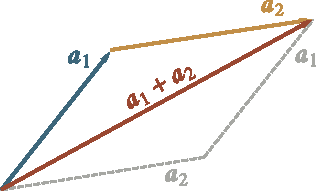
\includegraphics[scale=0.95]{figures/ch_01/fig_1_5.pdf}
			\caption[]{}
			\label{fig:1_5}
		\end{center}
	\end{minipage}
	\hfill{ }%\hspace{-0.1cm}
	\begin{minipage}[t]{0.5\linewidth}
		\begin{center}
			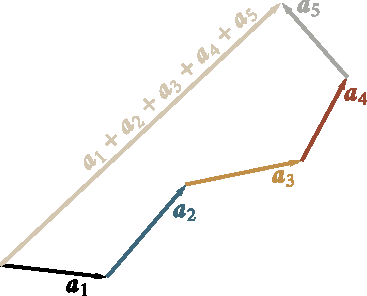
\includegraphics[scale=0.95]{figures/ch_01/fig_1_6.pdf}
			\caption[]{}
			\label{fig:1_6}
		\end{center}
	\end{minipage}
\end{figure}

Người ta gọi hiệu của hai vector $\vec{a}$ và $\vec{b}$ là một vector $\vec{c}$ mà khi cộng nó với $\vec{b}$ lại được vector $\vec{a}$ (\fig{1_7}---về vector $\vec{b}$ được biểu diễn bằng đường chấm chấm sẽ nói ở dưới). Chỉ có thể viết module của hai vector giống như module của tổng [xem \eqn{1_1}] bằng các vạch thẳng đứng:
\begin{equation}\label{eq:1_2}
|\vec{a}_1 - \vec{a}_2| = \text{module của vector } (\vec{a}_1 - \vec{a}_2),
\end{equation}

\noindent
vì ký hiệu $a_1-a_2$ là hiệu các module của các vector $\vec{a_1}$ và $\vec{a_2}$ mà nói chung không bằng không bằng module của hiệu.

\textbf{Phép nhân một vector với một vô hướng.} Kết quả nhân vector $\vec{a}$ với vô hướng $\alpha$ ta được vector mới $\vec{b}=\alpha$ có module lớn gấp $|\alpha|$ lần module của vector $\vec{a}$ ($b=|\alpha|a$). Chiều của vector $\vec{b}$ hoặc trùng với chiều của vector $\vec{a}$ (nếu $\alpha>0$), hoặc ngược với chiều của vector $\vec{a}$ (nếu $\alpha<0$). Từ điều đã nói trên suy ra rằng, phép nhân với $-1$ sẽ đổi ngược chiều của vector. Do đó các vector $\vec{a}$ và $-\vec{a}$ có các module như nhau nhưng ngược về chiều. Theo \fig{1_7} dễ dàng khẳng định rằng phép trừ vector $\vec{a}$ với vector $\vec{b}$ tương đương với việc thêm vector $\vec{-b}$ và vector $\vec{a}$.

Từ định nghĩa về phép toán nhân một vector với một vô hướng suy ra rằng mọi vector $\vec{a}$ có thể biểu diễn dưới dạng
\begin{equation}\label{eq:1_3}
\vec{a} = a\,\vecuni{a},
\end{equation}

\noindent
trong đó $a$ là module của vector $\vec{a}$, $\vecuni{a}$là vector có module bằng đơn vị và cùng chiều với vector $\vec{a}$ (\fig{1_8}).

Vector $\vecuni{a}$ được gọi là \textbf{vector đơn vị} hoặc là \textbf{chuẩn} của vector $\vec{a}$. Có thể biểu diễn chuẩn dưới dạng
\begin{equation}\label{eq:1_4}
\vecuni{a} = \frac{\vec{a}}{a},
\end{equation}

\noindent
từ đó suy ra rằng chuẩn là một đại lượng không có thứ nguyên.

\begin{figure}[!htb]
	\begin{minipage}[t]{0.5\linewidth}
		\begin{center}
			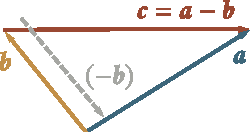
\includegraphics[scale=0.9]{figures/ch_01/fig_1_7.pdf}
			\caption[]{}
			\label{fig:1_7}
		\end{center}
	\end{minipage}
	\hfill{ }%\hspace{-0.1cm}
	\begin{minipage}[t]{0.5\linewidth}
		\begin{center}
			
\includegraphics[scale=0.95]{figures/ch_01/fig_1_8.pdf}
			\caption[]{}
			\label{fig:1_8}
		\end{center}
	\end{minipage}
\end{figure}

Có thể đưa ra các chuẩn không chỉ cho các vector mà cả cho các hướng bất kỳ trong không gian. Chẳng hạn như $\vecuni{x}$ là chuẩn của trục tọa độ $x$, $\vecuni{n}$ là chuẩn của pháp tuyến của đường hoặc mặt cong, and $\vecuni{\tau}$ là chuẩn của tiếp tuyến của đường cong.

\textbf{Sự phụ thuộc tuyến tính giữa các vector.} Ta hãy xét ba vector không đồng phương $\vec{a}$, $\vec{b}$ và $\vec{c}$ nằm trên một mặt phẳng. Từ \fig{1_9} rõ ràng là một vector bất kỳ trong chúng ($\vec{c}$ chẳng hạn) có thể được biểu diễn qua hai vector kia nhờ hệ thức
\begin{equation}\label{eq:1_5}
\vec{c} = \alpha\vec{a} + \beta\vec{b},
\end{equation}

\noindent
trong đó $\alpha$ và $\beta$ là các số nào đó (đối với trường hợp trình bày trên hình: $\alpha>1$, $-1<\beta<0$). Từ đó ta kết luận rằng vector $\vec{c}$ bất kỳ nằm trong một mặt phẳng với các vector không đồng phương, $\vec{a}$ và $\vec{b}$ có thể được biểu diễn qua các vector này nhờ hệ thức tuyến tính\eqref{eq:1_5}. Với các vector cố định $\vec{a}$ và $\vec{b}$ một vector thứ ba bất kỳ được xác định đơn trị bằng hai đại lượng $\alpha$ và $\beta$.

Giả sử cho ba vector $\vec{a}$, $\vec{b}$, $\vec{c}$ mà từng vector trong chúng không đồng phẳng với hai vector còn lại\footnote{Hai vector là luôn luôn đồng phẳng. Điều này suy ra từ chỗ là có thể làm trùng gốc của chúng bằng một sự dịch chuyển song song. Khi đó chúng được đặt trong một mặt phẳng.} Tương tự như \eqn{1_5} dễ dàng đoán ra rằng vector $\vec{d}$ bất kỳ có thể biểu diễn như một tổ hợp tuyến tính của các vector đã cho:
\begin{equation}\label{eq:1_6}
\vec{d} = \alpha\vec{a} + \beta\vec{b} + \gamma\vec{c},
\end{equation}

\noindent
Với các vector cố định $\vec{a}$, $\vec{b}$ và $\vec{c}$ vector $\vec{d}$ bất kỳ được xác định đơn trị bằng ba đại lượng $\alpha$, $\beta$ và $\gamma$, mà từng đại lượng có thể hoặc dương hoặc âm.

\textbf{Hình chiếu của một vector.} Ta xét một hướng nào đó trong không gian mà ta quy định là trục $l$ (\fig{1_10}). Giả thử vector $\vec{a}$ tạo với trục $l$ một góc $\varphi$ $l$\footnote{Nếu một đường thẳng mà vector $\vec{a}$ luôn hướng dọc theo đó và trục $l$ không cắt nhau thì để xác định góc $\varphi$ cần phải lấy một đường thẳng song song với vector $\vec{a}$ và cắt trục $l$. Góc giữa đường thẳng này và trục $l$ sẽ là góc $\varphi$ mà ta cần đến.}. Đại lượng
\begin{equation}\label{eq:1_7}
a_l = a\, \cos\varphi
\end{equation}

\noindent
($a$ là module của vector) được gọi là hình chiếu của vector $\vec{a}$ trên trục $l$.Hình chiếu được ký hiệu cùng một chữ như vector có thêm một chi số chỉ hướng mà vector được chiếu lên đó.

\begin{figure}[!htb]
	\begin{minipage}[htb!]{0.5\linewidth}
		\begin{center}
			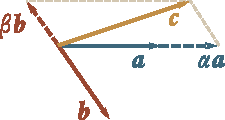
\includegraphics[scale=1]{figures/ch_01/fig_1_9.pdf}
			\caption[]{}
			\label{fig:1_9}
		\end{center}
	\end{minipage}
	\hfill{ }%\hspace{-0.1cm}
	\begin{minipage}[htb!]{0.5\linewidth}
		\begin{center}
			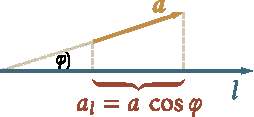
\includegraphics[scale=0.95]{figures/ch_01/fig_1_10.pdf}
			\caption[]{}
			\label{fig:1_10}
		\end{center}
	\end{minipage}
\end{figure}

Hình chiếu của vector là một đại lượng đại số. Nếu vector tạo với chiều đã cho một góc nhọn thì $\cos\varphi>0$, cho nên hình chiếu là dương. Nếu góc $\varphi$ là góc tù thì $\cos\varphi<0$ và do đó hình chiếu là âm. Khi vector vuông góc với trục đã cho thì hình chiếu bằng không. 

Hình chiếu của vector có một ý nghĩa hình học đơn giản. Nó bằng khoảng cách giữa các hình chiếu lên trục của gốc và ngọn của đoạn thẳng biểu diễn vector đã cho. Trong trường hợp $\varphi<\pi/2$ thì khoảng cách này lấy dâu cộng, trong trường hợp $\varphi>\pi/2$, nó lấy dấu trừ.

Giả thử $\vec{a} = \vec{a}_1+\vec{a}_2+\vec{a}_3+\vec{a}_4$ (\fig{1_11}). Từ hình vẽ dễ dàng kết luận rằng hình chiếu của vector tổng a lên một hướng nào đó bằng tổng hình chiếu của các vector số hạng:
\begin{equation}\label{eq:1_8}
a_l = a_{1l}+a_{2l}+a_{3l}+a_{4l}.
\end{equation}

\noindent
Ta hãy nhớ rằng, khi lấy tổng các hình chiếu của các vector biểu diễn trên \fig{1_11}, cần phải lấy các khoảng cách $0$---$1$, $1$---$2$, và $2$---$3$ với dấu cộng còn khoảng cách $3$---$4$ lấy dấu trừ. Công thức \eqref{eq:1_8} vẫn đúng với một số bất kỳ các số hạng.

\textbf{Biểu diễn vector qua các hình chiều của nó lên các trục tọa độ.} Ta hãy lấy các trục tọa độ Descartes và xét một vector $\vec{a}$ nằm trong mặt phẳng vuông góc với trục $z$ (\fig{1_12}). Ta hãy đưa vào các chuẩn của các trục tọa độ, tức là các vector đơn vị $\vecuni{x}$, $\vecuni{y}$, $\vecuni{z}$ ($\vecuni{z}$ không được vẽ trên hình, nó vuông góc với mặt phẳng của hình vẽ và hướng về phía chúng ta). Ta hãy chú ý rằng bộ ba chuẩn này hoàn toàn xác định hệ tọa độ và do đó được gọi là \textbf{cơ sở của hệ tọa độ}.

\begin{figure}[!htb]
	\begin{minipage}[t]{0.5\linewidth}
		\begin{center}
			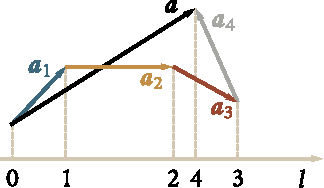
\includegraphics[scale=1]{figures/ch_01/fig_1_11.pdf}
			\caption[]{}
			\label{fig:1_11}
		\end{center}
	\end{minipage}
	\hfill{ }%\hspace{-0.1cm}
	\begin{minipage}[t]{0.5\linewidth}
		\begin{center}
			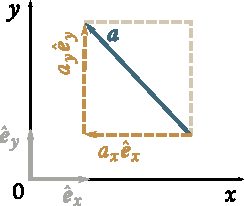
\includegraphics[scale=0.95]{figures/ch_01/fig_1_12.pdf}
			\caption[]{}
			\label{fig:1_12}
		\end{center}
	\end{minipage}
\end{figure}

Từ \fig{1_12} rõ ràng có thể biểu diễn vector $\vec{a}$ dưới dạng một tổ hợp tuyến tính chuẩn $\vecuni{x}$ và $\vecuni{y}$ [xem \eqn{1_5}]:
\begin{equation*}
\vec{a} = a_x \vecuni{x} + a_y \vecuni{y}.
\end{equation*}

\noindent
Các hình chiếu của vector lên các trục tọa độ đóng vai trò các hệ số $\alpha$ và $\beta$. Trong ví dụ được xét, hình chiếu $a_x$ là âm, do đó vector $a_x\vecuni{x}$ có chiều ngược lại với chiều của chuẩn $\vecuni{x}$.

Ta đã lấy vector $\vec{a}$ vuông góc với trục $z$, do đó vector $a_z=0$. Trong trường hợp tổng quát khi tất cả ba hình chiếu của vector đều khác không:
\begin{equation}\label{eq:1_9}
\vec{a} = a_x \vecuni{x} + a_y \vecuni{y} + a_z \vecuni{z},
\end{equation}

\noindent
Như vậy, có thể biểu diễn một vector bất kỳ quá các hình chiếu của nó lên các trục tọa độ được gọi là \textbf{các thhành phần} của vector.

Các đại lượng $a_x$, $a_y$, $a_z$ bằng (chính xác đến dấu) các cạnh của một hình hộp chữ nhật mà đường chéo lơn của nó là vector $\vec{a}$ (\fig{1_13}). Do đó có hệ thức
\begin{equation}\label{eq:1_10}
a^2 = a_x^2 + a_y^2 + a_z^2.
\end{equation}

Giả thử $\vec{c}=\vec{a}+\vec{b}$. Biểu diễn từng vector theo đúng công thức \eqn{1_9}, ta có
\begin{equation*}
c_x\vecuni{x} + c_y\vecuni{y} + a_z\vecuni{z} = (a_x+b_x)\vecuni{x} + (a_y+b_y)\vecuni{y} + (a_z+b_z)\vecuni{z}
\end{equation*}

\noindent
(ta đưa ra ngoài các dấu ngoặc các thừa số chung $\vecuni{x}$, $\vecuni{y}$ và $\vecuni{z}$)· Các vector bằng nhau đều có các hình chiếu bằng nhau trên các trục tọa độ. Trên cơ sở này có thể viết là
\begin{equation}\label{eq:1_11}
c_x=a_x+b_x,\quad c_y=a_y+b_y,\quad a_z=a_z+b_z
\end{equation}

\noindent
[so sánh với \eqn{1_8}]. Các công thức \eqref{eq:1_11} là biểu thúc giải tích của qui tắc cộng các vector. Chúng đúng với một số bất kỳ các số hạng

\textbf{Bán kính vector.} Người ta gọi bán kính vector $\vec{r}$ của một điểm nào đó là một vector vẽ từ gốc tọa độ tới điểm đã cho (\fig{1_14}). Các hình chiếu của nó lên các trục tọa độ đều bằng các tọa độ Descartes của điểm đã cho:
\begin{equation}\label{eq:1_12}
r_x=x,\quad r_y=y,\quad r_z=z.
\end{equation}

\noindent
Do đó, ứng với \eqn{1_9} có thể biểu diễn bán kính vector dưới dạng
\begin{equation}\label{eq:1_13}
\vec{r} = x\vecuni{x} + y\vecuni{y} + z\vecuni{z}.
\end{equation}

\noindent
Theo \eqn{1_10}
\begin{equation}\label{eq:1_14}
r^2 = x^2 + y^2 + z^2.
\end{equation}

\begin{figure}[!htb]
	\begin{minipage}[t]{0.5\linewidth}
		\begin{center}
			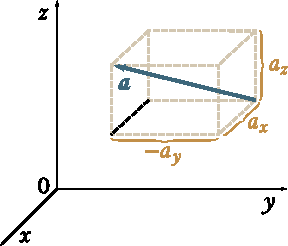
\includegraphics[scale=1]{figures/ch_01/fig_1_13.pdf}
			\caption[]{}
			\label{fig:1_13}
		\end{center}
	\end{minipage}
	\hfill{ }%\hspace{-0.1cm}
	\begin{minipage}[t]{0.5\linewidth}
		\begin{center}
			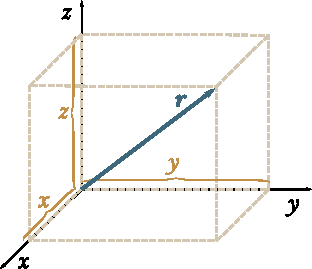
\includegraphics[scale=0.95]{figures/ch_01/fig_1_14.pdf}
			\caption[]{}
			\label{fig:1_14}
		\end{center}
	\end{minipage}
\end{figure}

\textbf{Tích vô hướng của các vector.} Có thể nhân hai vector $\vec{a}$ và $\vec{b}$ với nhau theo hai cách, một cách dẫn tới đại lượng vô hướng, cách kia cho kết quả là một vector mới nào đó. Ứng với điều này có hai tích của các vector---tích vô hướng và tích vector. Ta hãy chú ý rằng \textit{không có phép tính chia một vector cho một vector}.

Người ta gọi tích vô hướng của các vector $\vec{a}$ và $\vec{b}$ là một vô hướng bằng tích các module của các vector này với cos của góc $\alpha$ giữa chúng:
\begin{equation}\label{eq:1_15}
\vecdot{a}{b} = ab\cos\alpha
\end{equation}

\noindent
(\fig{1_15}). When writing a scalar product, the symbols of the vectors being multiplied are usually written next to each other with dot between them (this is why a scalar product is also called a dot product; sometimes nothing is used between the symbols)\footnote{The dot symbol between vectors is preferred in the \LaTeX version to adopt a more modern approach.}. Equation~\eqref{eq:1_15} expresses an algebraic quantity: when $\alpha$ is acute, we have $\vecdot{a}{b}>0$, and when it is obtuse, we have $\vecdot{a}{b}<0$. The scalar product of mutually perpendicular vectors ($\alpha=\pi/2$) equals zero.

\begin{figure}[!htb]
	\begin{center}
		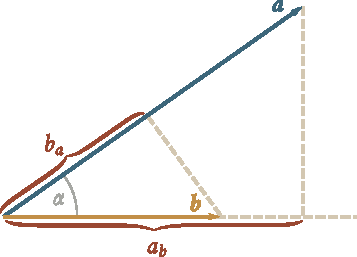
\includegraphics[scale=0.9]{figures/ch_01/fig_1_15.pdf}
		\caption[]{}
		\label{fig:1_15}
	\end{center}
\end{figure}

Ta hãy chú ý rằng bình phương của một vector luôn luôn được hiểu ngầm là tích vô hướng của vector với chính nó:
\begin{equation}\label{eq:1_16}
\vec{a}^2 = \vecdot{a}{a} = aa\cos\alpha = a^2.
\end{equation}

\noindent
Như vậy bình phương của một vector bằng bình phương module của nó. Đặc biệt là bình phương của một chuẩn bất kỳ bằng đơn vị:
\begin{equation}\label{eq:1_17}
\vecuni{x}^2 = \vecuni{y}^2 = \vecuni{z}^2 = 1.
\end{equation}

\noindent
Đồng thời ta hãy chú ý rằng do các chuẩn vuông góc với nhau nên các tích vô hướng có dạng $\vecunidot{i}{k}$ đều bằng không, nếu $i\neq k$.

Dùng ký hiệu Kronecker $\delta_{ik}$ được định nghĩa như sau:
\begin{equation}\label{eq:1_18}
\delta_{ik} = \begin{cases}
1, &\mbox{if } i = k, \\
0, &\mbox{if } i\neq k. \end{cases}
\end{equation}
là rất tiện lợi.

\noindent
Nếu sử dụng ký hiệu này thì có thể biểu thị các tính chất đã thiết lập ở trên của các tích vô hướng các chuẩn của các trục tọa độ bằng một công thức:
\begin{equation}\label{eq:1_19}
\vecunidot{i}{k} = \delta_{ik}\quad (i, k = x, y, z)
\end{equation}

\noindent
(các chỉ số $i$ và $k$ có thể lấy các giá trị $x$, $y$ và $z$ độc lập với nhau).

Từ định nghĩa \eqref{eq:1_15} suy ra rằng, tích vô hướng có tính giao hoán, nghĩa là không phụ thuộc vào thứ tự các nhân tử:
\vspace{-12pt}
\begin{equation}\label{eq:1_20}
\vecdot{a}{b} = \vecdot{b}{a}.
\end{equation}

\noindent
Có thể viết biểu thức \eqref{eq:1_15} theo một số cách:
\begin{equation*}
\vecdot{a}{b} = ab\cos\alpha = (a\cos\alpha)\,b = a\,(b\cos\alpha).
\end{equation*}

\noindent
Từ \fig{1_15} rõ ràng là $a\cos\alpha$ bằng $a_b$ là hình chiếu của vector $\vec{a}$ lên hướng của vector $\vec{b}$. Một cách tương tự, $b\cos\alpha= b_a$ là hình chiếu của vector $\vec{b}$ lên hướng của vector $\vec{a}$. Do đó có thể nói rằng, người ta gọi tích vô hướng của hai vector là một vô hướng bằng tích module của một vector nhân tử với hình chiếu của vector kia lên hướng của vector này:
\begin{equation}\label{eq:1_21}
\vecdot{a}{b} = a_b b = a b_a.
\end{equation}

Nếu để ý rằng hình chiếu của tổng các vector bằng tổng các hình chiếu của các vector số hạng thì ta có thể viết:
\begin{equation}\label{eq:1_22}
\vec{a}\boldsymbol{\cdot}(\vec{b}+\vec{c}+\ldots) = a(\vec{b}+\vec{c}+\ldots)_a = a(b_a+c_a+\ldots) = ab_a+ac_a+\ldots = ab+ac+\ldots .
\end{equation}

\noindent
Từ đó suy ra rằng tích vô hướng của các vector có tính phân phối, nghĩa là tích của vector $\vec{a}$ với tổng một số vector bằng tổng các tích của vector $\vec{a}$ với mỗi vector số hạng được lấy tách biệt.

Biểu diễn các vector nhân tử dưới dạng \eqn{1_9} và sử dụng tính phân phối của tích vô hướng, ta có:
\begin{align*}
\vecdot{a}{b} &= (a_x\vecuni{x} + a_y\vecuni{y} + a_z\vecuni{z})(b_x\vecuni{x} + b_y\vecuni{y} + b_z\vecuni{z})\\
&= a_xb_x\vecunidot{x}{x} + a_xb_y\vecunidot{x}{y} + a_xb_z\vecunidot{x}{z} + a_yb_x\vecunidot{y}{x} + a_yb_y\vecunidot{y}{y}\\
&\,+ a_yb_z\vecunidot{y}{z}+ a_zb_x\vecunidot{z}{x} + a_zb_y\vecunidot{z}{y} + a_zb_z\vecunidot{z}{z}.
\end{align*}

\noindent
Bây giờ hãy chú ý đến \eqn{1_19}. Kết quả là ta được biểu thức của tích vô hướng qua các hình chiếu của các vector nhân tử:
\begin{equation}\label{eq:1_23}
\vecdot{a}{b} = a_xb_x + a_yb_x + a_zb_z.
\end{equation}

\noindent
Ta chú ý rằng khi quay các trục tọa độ thì các hình chiếu của các vector trên các trục này sẽ bị biến đổi. Tuy nhiên đại lượng $ab\cos\alpha$ không phụ thuộc vào việc chọn trục. Từ đó ta kết luận rằng các biến đổi hình chiếu của các vector $\vec{a}$ và $\vec{b}$ khi quay các trục mang một đặc tính là tổ hợp của chúng có dạng \eqn{1_23} vẫn bất biến (không biến đổi):
\begin{equation}\label{eq:1_24}
\vecdot{a}{b} = a_xb_x + a_yb_x + a_zb_z = \mathrm{inv}.
\end{equation}

Dễ dàng hiểu được rằng có thể biểu diễn hình chiếu của vector $\vec{a}$ lên hướng $l$ [xem \eqn{1_7}] dưới dạng
\begin{equation}\label{eq:1_25}
a_l = \vec{a}\boldsymbol{\cdot}\vecuni{l},
\end{equation}

\noindent
trong đó $\vecuni{l}$ là chuẩn của hướng $l$. Một cách tương tự,
\begin{equation}\label{eq:1_26}
a_x = \vec{a}\boldsymbol{\cdot}\vecuni{x},\quad  a_y = \vec{a}\boldsymbol{\cdot}\vecuni{y}, \quad  a_z=\vec{a}\boldsymbol{\cdot}\vecuni{z}.
\end{equation}

\textbf{Tích vector.} Người ta gọi vector $\vec{c}$ được xác định bằng công thức
\begin{equation}\label{eq:1_27}
\vec{c} = ab\sin(\alpha)\hatvec{n},
\end{equation}
là tích vector của các vector $\vec{a}$ và $\vec{b}$.

\noindent
Trong đó $a$ và $b$ là các module của các vector nhân tử, $\alpha$ là góc ở giữa các vector, $\hatvec{n}$ là vector đơn vị của pháp tuyến\footnote{Ký hiệu $\hatvec{n}$ đơn giản hơn và trực quan hơn là $\vecuni{n}$.} với mặt phẳng chứa các vector $\vec{a}$ và $\vec{b}$ (\fig{1_16}).

Chiều của $\hatvec{n}$ được chọn sao cho dãy các vector $\vec{a}$, $\vec{b}$, $\hatvec{n}$ tạo thành một hệ đinh ốc thuận. Điều này có nghĩa là nếu nhìn theo vector $\hatvec{n}$ thì phép quay theo con đường ngắn nhất từ nhân tử thứ nhất tới nhân tử thứ hai được thực hiện theo chiều quay của kim đồng hồ. Trên \fig{1_16}, vector $\hatvec{n}$ hướng ra sau hình vẽ và do đó được biểu diễn bằng một vòng tròn nhỏ có dấu chữ thập\footnote{Chúng ta sẽ biểu diễn các vector vuông góc với mặt phẳng hình vẽ bằng một vòng tròn nhỏ có dấu chữ thập nếu vector hướng ra xa ta, và bằng một vòng tròn nhỏ có điểm chấm ở tâm nếu vector hướng về ta. Để dễ thấy, có thể hình dung một vector dưới dạng một mũi tên với phần đầu có dạng hình nón và phần đuôi có dạng hình chữ thập. Khi đó nếu vector hướng về phía chúng ta (mũi tên bay tới chúng ta), ta sẽ nhìn thấy một vòng tròn nhỏ với điểm chấm, nếu cũng vector đó hướng ra xa chúng ta (mũi tên bay ra xa ta), ta sẽ nhìn thấy một vòng tròn với dấu chữ thập.}. Hướng của vector $\vec{c}$ trùng với hướng của $\hatvec{n}$.

\begin{figure}[!htb]
	\begin{center}
		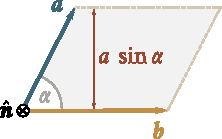
\includegraphics[scale=1]{figures/ch_01/fig_1_16.pdf}
		\caption[]{}
		\label{fig:1_16}
	\end{center}
\end{figure}

Có thể viết một cách tượng trưng tích vector theo hai cách:
\begin{equation*}
[\vec{a},\vec{b}]\quad\text{hoặc}\quad \vec{a}\times\vec{b}
\end{equation*}

\noindent
the latter notation resulting in the term cross product sometimes being used to signify a vector product. We shall use the latter notation\footnote{To avoid confusion, in the \LaTeX version, we shall use the cross product symbol.}. Thus, according to \eqn{1_27}, we have
\begin{equation}\label{eq:1_28}
\vecprod{a}{b} = (ab\sin\alpha)\hatvec{n}.
\end{equation}

Từ \fig{1_16} rõ ràng là module của vector tích có ý nghĩa hình học đơn giản---biểu thức $ab\sin\alpha$ về trị số bằng điện tích hình bình hành tạo bởi các vector nhân tử.

Chúng ta đã xác định hướng của vector $\vecprod{a}{b}$ bằng cách liên kết nó với chiều quay từ nhân tử thứ nhất tới nhân tử thứ hai. Khi khảo sát các vector như bán kính vector $\vec{r}$, vận tốc $\vec{v}$, lực $\vec{F}$,...vấn đề chọn hướng của chúng không đặt ra vì nó suy ra một cách tự nhiên từ bản chất của chính các đại lượng. Các vector như thế được gọi là các \textbf{vector thực} (hoặc các vector cực). Các vector loại $\vecprod{a}{b}$ có chiều liên kết với chiều quay được gọi là \textbf{giả vector} (hoặc các vector trục). Khi thay đổi điều kiện, chẳng hạn khi chuyển từ hệ tọa độ thuận sang hệ tọa độ nghịch, chiều của các giả vector biến đổi ngược lại, trong lúc đó các vector thực vẫn không biến đổi.

Cần chú ý rằng tích vector sẽ là một giả vector chỉ trong trường hợp khi cả hai vector nhân tử đều là các vector thực (hoặc cả hai đều là các giả vector). Tích vector của một vector thực với một giả vector sẽ là một vector thực. Sự thay đổi ngược lại điều kiện xác định chiều của các giả vector trong trường hợp này dẫn tới sự đổi dấu đứng trước tích vector và đồng thời dẫn tới sự đổi dấu đứng trước một trong các nhân tử. Rốt cuộc là đại lượng được biểu thị bằng tích vector vẫn không đổi.

Vì chiều của tích vector được xác định bằng chiều quay từ nhân tử thú nhất tới nhân tử thứ hai nên kết quả của phép nhân vector phụ thuộc vào thứ tự của các nhân tử. Sự hoán vị các nhân tử gây ra sự đổi ngược lại chiều của vector kết quả. Như vậy, tích vector không có tính chất giao hoán:
\begin{equation}\label{eq:1_29}
\vecprod{a}{b} = -\vecprod{b}{a}.
\end{equation}

\noindent
Có thể chứng minh rằng tích vector có tính phân phối, nghĩa là
\begin{equation}\label{eq:1_30}
\vec{a}\times(\vec{b}_1+\vec{b}_2+\ldots)] = \vec{a}\times\vec{b}_1 + \vec{a}\times\vec{b}_2 + \ldots.
\end{equation}

\begin{figure}[!htb]
	\begin{center}
		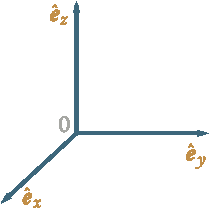
\includegraphics[scale=1]{figures/ch_01/fig_1_17.pdf}
		\caption[]{}
		\label{fig:1_17}
	\end{center}
\end{figure}

Ta hãy xét các tích vector của các chuẩn của các trục tọa độ (\fig{1_17}). Theo định nghĩa \eqref{eq:1_28}
\begin{align}
\vecuniprod{x}{x} &= \vecuniprod{y}{y} = \vecuniprod{z}{z} = 0,\nonumber\\
\vecuniprod{x}{y} &= -\vecuniprod{y}{x} = \vecuni{z},\label{eq:1_31}\\
\vecuniprod{y}{z} &= -\vecuniprod{z}{y} = \vecuni{x},\nonumber\\
\vecuniprod{z}{x} &= -\vecuniprod{x}{z} = \vecuni{y}.\nonumber
\end{align}

\noindent
Biểu diễn các vector dưới dạng \eqn{1_9} và sử dụng tính phân phối của tích vector ta có:
\begin{align*}
\vecprod{a}{b} &= (a_x\vecuni{x}+a_y\vecuni{y}+a_z\vecuni{z})\times(b_x\vecuni{x}+b_y\vecuni{y}+b_z\vecuni{z})\\
&= a_xb_x\vecuniprod{x}{x} + a_xb_y\vecuniprod{x}{y} + a_xb_z\vecuniprod{x}{z}\\
&+ a_yb_x\vecuniprod{y}{x} + a_yb_y\vecuniprod{y}{y} + a_yb_z\vecuniprod{y}{z}\\
&+ a_zb_x\vecuniprod{z}{x} + a_zb_y\vecuniprod{z}{y} + a_zb_z\vecuniprod{z}{z}
\end{align*}

\noindent
Nếu chú ý đến hệ thức \eqref{eq:1_31}, ta đi tới biểu thức sau:
\begin{equation}\label{eq:1_32}
\vecprod{a}{b} = \vecuni{x}(a_yb_z - a_zb_y) + \vecuni{y}(a_zb_x - a_xb_z) + \vecuni{z}(a_xb_y - a_yb_x).
\end{equation}

\noindent
Có thể biểu diễn biểu thức thu được dưới dạng định thức:
\vspace{-12pt}
\begin{equation}\label{eq:1_33}
\vecprod{a}{b} = \begin{vmatrix}
\vecuni{x} & \vecuni{y} & \vecuni{z}\\
a_x & a_y & a_z\\
b_x & b_y & b_z
\end{vmatrix}.
\end{equation}

\textbf{Tích hỗn hợp.} Biểu thức $\vecmix{a}{b}{c}$ được gọi là tích hỗn hợp (hoặc tích vô hướng-vector) của ba vector, nghĩa là tích vô hướng của vector $\vec{a}$ với tích vector của các vector $\vec{b}$ và $\vec{c}$. Theo các định nghĩa \eqref{eq:1_15} và \eqref{eq:1_28}
\begin{equation*}
\vecmix{a}{b}{c} = a\{bc\sin(\vec{b}, \vec{c})\}\cos(\vec{a},\hatvec{n}).
\end{equation*}

\begin{figure}[!htb]
	\begin{center}
		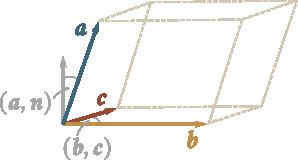
\includegraphics[scale=1]{figures/ch_01/fig_1_18.pdf}
		\caption[]{}
		\label{fig:1_18}
	\end{center}
\end{figure}

\noindent
Ở đây $(\vec{b},\vec{c})$ là góc giữa $\vec{b}$ và $\vec{c}$, $(\vec{a},\hatvec{n})$ là góc giữa vector $\vec{a}$ và chuẩn $\hatvec{n}$ xác định $\vecprod{b}{c}$. Từ \fig{1_18} rõ ràng là biểu thức $bc\sin(\vec{b},\vec{c})$ về trị số bằng diện tích đáy của hình hộp được tạo bởi các vector nhân tử còn biểu thức $a\cos(\vec{a},\hatvec{n})$ về trị số bằng chiều cao của hình hộp này lấy với dấu cộng nếu góc $(\vec{a},\hatvec{n})$ là nhọn và với dấu trừ nếu góc này là tù. Do đó biểu thức $\vecmix{a}{b}{c}$ có ý nghĩa hình học đơn giản---về trị số nó bằng thể tích của hình hộp được tạo bởi các vector nhân tử [lấy dấu cộng hay trừ tùy theo độ lớn của góc $(\vec{a},\hatvec{n})$]. Khi tính thể tích của hình hộp, kết quả không thể phụ thuộc vào điều là mặt nào trong các mặt của nó được lấy làm đáy. Từ đó suy ra rằng
\begin{equation}\label{eq:1_34}
\vecmix{a}{b}{c} = \vecmix{b}{c}{a} = \vecmix{c}{a}{b}.
\end{equation}

\noindent
Như vậy, tích hỗn hợp cho phép hoán vị vòng quanh các nhân tử, nghĩa là cho phép thay thế mỗi nhân tử tiếp sau đó theo chu trình:
\begin{equation*}
% \begin{tikzcd}
% \vec{a}\arrow[rd] &\\
% \vec{c}\arrow[u] & \arrow[l] \vec{b}
% \end{tikzcd}
\begin{tikzcd}[column sep=small]
             & \vec{a} \arrow[rd] &              \\
\vec{c} \arrow[ru] &              & \vec{b} \arrow[ll]
\end{tikzcd}
\end{equation*}

\textbf{Tích vector kép.} Ta hãy nghiên cứu tích vector kép của vector $\vec{a}$, $\vec{b}$ và $\vec{c}$
\begin{equation*}
\vec{d} = \vec{a}\times\vecprod{b}{c}.
\end{equation*}

\noindent
Mỗi tích vector là vuông góc với cả hai nhân tử. Do đó vector $\vec{d}$ vuông góc với chuẩn $\hatvec{n}$ xác định hướng của vector $\vecprod{b}{c}$. Từ đó suy ra rằng vector $\vec{d}$ nằm trong mặt phẳng tạo bởi các vector $\vec{b}$ và $\vec{c}$, và do đó có thể được biểu diễn như một tổ hợp tuyến tính của các vector này:
\begin{equation*}
\vec{d} = \alpha\vec{b} + \beta\vec{c}
\end{equation*}

\noindent
[xem \eqn{1_5}]. Phép tính toán tương ứng cho $\alpha=\vecdot{a}{c}$, $\beta=-\vecdot{a}{b}$. Như vậy
\begin{equation}\label{eq:1_35}
\vec{a}\times\vecprod{b}{c} = \vec{b}(\vecdot{a}{c}) - \vec{c}(\vecdot{a}{b}).
\end{equation}

\textbf{Đạo hàm của vector.} Ta hãy nghiên cứu một vector biến đổi theo thời gian theo một quy luật đã biết $\vec{a}(t)$. Hình chiếu của vector này trên các trục tọa độ là các hàm độ cho của thời gian. Do đó
\begin{equation}\label{eq:1_36}
\vec{a}(t) = \vecuni{x}a_x(t) + \vecuni{y}a_y(t) + \vecuni{z}a_z(t)
\end{equation}

\noindent
(ta giả thiết rằng các thục tọa độ không quay trong không gian, cho nên các chuẩn của các trục không biến đổi theo thời gian).

Giả thử trong khoảng thời gian $\Delta t$, các hình chiếu của vector nhận các số gia $\Delta a_x$, $\Delta a_y$, $\Delta a_z$. Khi đó vector nhận số gia $\Delta\vec{a} = \vecuni{x}\Delta a_x + \vecuni{y}\Delta a_y + \vecuni{z}\Delta a_z$. Có thể đặc trưng vận tốc biển đổi của vector $\vec{a}$ theo giời gian bằng tỷ số giữa $\Delta\vec{a}$ và $\Delta t$:
\begin{equation}\label{eq:1_37}
\frac{\Delta\vec{a}}{\Delta t} = \vecuni{x}\frac{\Delta a_x}{\Delta t} + \vecuni{y}\frac{\Delta a_y}{\Delta t} + \vecuni{z}\frac{\Delta a_z}{\Delta t}.
\end{equation}

\noindent
Tỷ số này cho vận tốc biển đổi trung bình của $\vec{a}$ trong khoảng thời gian $\Delta t$. Ta hãy giả thử rằng $\vec{a}$ biến đổi theo thời gian một cách liên tục mà không có các đột biến. Khi đó khoảng thời gian $\Delta t$ càng nhỏ thì đại lượng \eqn{1_37} càng đặc trưng chính xác hơn cho vận tốc biến đổi của $\vec{a}$ tại thời điểm $t$ xảy ra trước khoảng $\Delta t$. Do đó vận tốc biến đổi của vector $\vec{a}$ tại thời điểm $t$ bằng giới hạn của tỷ số \eqn{1_37} có được khi giảm vô hạn $\Delta t$:
\begin{align}
\text{vận tốc biến đổi của }\vec{a} &= \lim_{\Delta t\to 0}\frac{\Delta\vec{a}}{\Delta t} \nonumber\\
&= \vecuni{x} \lim_{\Delta t\to 0}\frac{\Delta a_x}{\Delta t} + \lim_{\Delta t\to 0}\vecuni{y} \frac{\Delta a_y}{\Delta t} + \lim_{\Delta t\to 0}\vecuni{z} \frac{\Delta a_z}{\Delta t}.\label{eq:1_38}
\end{align}

Nếu có một hàm $f(t)$ nào đó của đối số $t$, thì giới hạn của tỷ số giữa số gia của hàm $\Delta f$ với số gia của đối số $\Delta t$ có được khi $\Delta t$ dần tới không được gọi là đạo hàm của hàm $f$ theo $t$ và được ký hiệu bằng ký hiệu $\diffin{f}{t}$. Do đó có thể viết biểu thức \eqref{eq:1_38} như sau:
\begin{equation}\label{eq:1_39}
\diff{\vec{a}}{t} = \vecuni{x}\diff{a_x}{t} + \vecuni{y}\diff{a_y}{t} + \vecuni{z}\diff{a_z}{t}.
\end{equation}

\noindent
Kết quả thu được có nghĩa là các hình chiếu của vector $\diffin{\vec{a}}{t}$ lên các trục tọa độ bằng đạo hàm theo thời gian của các vector $\vec{a}$:
\begin{equation}\label{eq:1_40}
\left(\diff{\vec{a}}{t}\right)_{\text{pr. }x} = \diff{a_x}{t},\quad \left(\diff{\vec{a}}{t}\right)_{\text{pr. }y} = \diff{a_y}{t},\quad \left(\diff{\vec{a}}{t}\right)_{\text{pr. }z} = \diff{a_z}{t},\quad.
\end{equation}

Trong vật lý người ta thường ký hiệu các đạo hàm theo thời gian bằng ký hiệu của đại lượng tương ứng với một dấu chấm ở trên nó, chẳng hạn
\begin{equation}\label{eq:1_41}
\diff{\varphi}{t} = \dot{\varphi},\quad \diffsec{\varphi}{t} = \ddot{\varphi},\quad \diff{\vec{a}}{t} = \dot{\vec{a}},\quad \diffsec{\vec{a}}{t} = \ddot{\vec{a}}.
\end{equation}

\noindent
Nếu sử dụng ký hiệu đó thì công thức \eqref{eq:1_39} có thể nhận dạng
\begin{equation}\label{eq:1_42}
\dot{\vec{a}} = \vecuni{x}\dot{a}_x + \vecuni{y}\dot{a}_y + \vecuni{z}\dot{a}_z.
\end{equation}

\noindent
Nếu lấy bán kính vector $\vec{r}(t)$ của điểm chuyển động để làm $\vec{a}(t)$ thì theo \eqn{1_42}
\begin{equation}\label{eq:1_43}
\dot{\vec{r}} = \vecuni{x}\dot{r}_x + \vecuni{y}\dot{r}_y + \vecuni{z}\dot{r}_z,
\end{equation}

\noindent
trong đó $x$, $y$, $z$ là các hàm của $x=x(t)$, $y=t(t)$, $z=z(t)$.

Biểu thức
\begin{equation}\label{eq:1_44}
\mathrm{d}f = f'\, \mathrm{d}t,
\end{equation}
được gọi là vi phân (``số gia'') của hàm $f(t)$.

\noindent
Trong đó $f'$ là đạo hàm của $f$ theo $t$.  Theo \eqn{1_39} vi phân (``số gia'') của vector $\vec{a}$ được xác định bằng công thức
\begin{equation}\label{eq:1_45}
\mathrm{d}\vec{a} = \vecuni{x}\mathrm{d}a_x + \vecuni{y}\mathrm{d}a_y + \vecuni{z}\mathrm{d}a_z.
\end{equation}

Đặc biệt là
\begin{equation}\label{eq:1_46}
\mathrm{d}\vec{r} = \vecuni{x}\mathrm{d}x + \vecuni{y}\mathrm{d}y + \vecuni{z}\mathrm{d}z.
\end{equation}

Ta hãy chú ý rằng trong một khoảng thời gian $\Delta t$ rất nhỏ nhưng hữu hạn, số gia của hàm xấp xỉ bằng
\begin{equation}\label{eq:1_47}
\Delta f \approx f'\Delta t = \diff{f}{t}\Delta t.
\end{equation}

\noindent
Tại giới hạn khi $\Delta t\to 0$, đằng thức gần đúng \eqref{eq:1_47} chuyển thành đẳng thức đúng \eqref{eq:1_44}.

Có thể viết công thức tương tự \eqref{eq:1_47} cả đối với hàm vector
\begin{equation}\label{eq:1_48}
\Delta\vec{a} \approx \diff{\vec{a}}{t}\Delta t.
\end{equation}

\textbf{Đạo hàm của tích các hàm.} Ta hãy nghiên cứu hàm $\vec{b}(t)$, nó bằng tích của hàm vô hướng $\varphi(t)$ và hàm vector $\vec{a}(t)$, $\vec{b}(t)=\varphi(t)\vec{a}(t)$, hoặc một cách ngắn gọn $\vec{b}=\varphi\vec{a}$. Ta hãy tìm số gia của hàm $\vec{b}$:
\begin{equation*}
\Delta\vec{b} = \Delta(\varphi\vec{a}) = (\varphi + \Delta\varphi)(\vec{a} + \Delta\vec{a}) - \varphi\vec{a} = \varphi\Delta\vec{a} + \vec{a}\Delta\varphi + \Delta\varphi\Delta\vec{a}.
\end{equation*}

\noindent
Nếu biêu diễn số gia của hàm dưới dạng \eqref{eq:1_47} và \eqref{eq:1_48}, ta có:
\begin{equation*}
\Delta\vec{b} \approx \varphi\diff{\vec{a}}{t}\Delta t + \vec{a}\diff{\varphi}{t}\Delta t + \diff{\varphi}{t}\diff{\vec{a}}{t}(\Delta t)^2
\end{equation*}

\noindent
từ đó
\begin{equation*}
\frac{\Delta\vec{b}}{\Delta t} \approx \varphi\diff{\vec{a}}{t} + \vec{a}\diff{\varphi}{t} + \diff{\varphi}{t}\diff{\vec{a}}{t}\Delta t.
\end{equation*}

\noindent
Tại giới hạn khi $\mathrm{d}t$ tiến tới không, đẳng thức gần đúng này trở thành đẳng thức chính xác. Như vậy
\begin{equation*}
\diff{\vec{b}}{t} = \lim_{\Delta t\to 0} \diff{\vec{b}}{t} =  \lim_{\Delta t\to 0} \left(\varphi\diff{\vec{a}}{t} + \vec{a}\diff{\varphi}{t} + \diff{\varphi}{t} \diff{\vec{a}}{t}\Delta t\right).
\end{equation*}

\noindent
Hai số hạng đầu không phụ thuộc vào $\Delta t$ và do đó khi chuyển tới giới hạn sẽ không bị biến đổi. Giới hạn của số hạng thứ ba bằng không. Do đó, sau khi thay $\vec{b}$ bằng $\varphi\vec{a}$, ta có:
\begin{equation}\label{eq:1_49}
\diff{(\varphi\vec{a})}{t} = \varphi\diff{\vec{a}}{t} + \vec{a}\diff{\varphi}{t} = \varphi\dot{\vec{a}}+\dot{\varphi}\vec{a}.
\end{equation}

Bây giờ ta hãy nghiên cứu đạo hàm của tích vô hướng của hai hàm vector $\vec{a}(t)$ và $\vec{b}(t)$. Số gia của tích này bằng:
\begin{align*}
\Delta(\vec{a}\vec{b}) &= (\vec{a} + \Delta\vec{a})(\vec{b} + \Delta\vec{b}) - \vec{a}\vec{b}\\
&= \vec{a}\Delta\vec{b} + \vec{b}\Delta\vec{a} + \Delta\vec{a}\Delta\vec{b} \\
&\approx \vec{a}\dot{\vec{b}}\Delta t + \vec{b}\dot{\vec{a}}\Delta t + \dot{\vec{a}}\dot{\vec{b}}(\Delta t)^2
\end{align*}

\noindent
Từ đó
\begin{equation*}
\diff{(\vec{a}\vec{b})}{t} = \lim_{\Delta t\to 0} \frac{\Delta(\vec{a}\vec{b})}{\Delta t} = \lim_{\Delta t\to 0} (\vec{a}\dot{\vec{b}} + \vec{b}\dot{\vec{a}} + \dot{\vec{a}}\dot{\vec{b}}\Delta t)
\end{equation*}

\noindent
hoặc cuối cùng
\begin{equation}\label{eq:1_50}
\diff{(\vec{a}\vec{b})}{t} = \vec{a}\dot{\vec{b}} + \vec{b}\dot{\vec{a}}.
\end{equation}

\noindent
Nhân \eqn{1_50} với $\mathrm{d}t$ ta có vi phân:
\begin{equation}\label{eq:1_51}
\diff{(\vec{a}\vec{b})}{t} = \vec{a}\dot{\vec{b}} + \vec{b}\dot{\vec{a}}.
\end{equation}

Ta hãy tính đạo hàm và vi phân của bình phương hàm vector. Theo \eqref{eq:1_50} và \eqref{eq:1_51}
\begin{align}
\diff{\vec{a}^2}{t} &= 2\vec{a}\dot{\vec{a}},\label{eq:1_52}\\
\mathrm{d}(\vec{a}^2) &= 2\vec{a}\,\mathrm{d}\vec{a},\label{eq:1_53}
\end{align}

\noindent
Nếu để ý rằng $\vec{a}^2 = a^2$ [xem \eqn{1_16}] thì có thể viết:
\begin{equation}\label{eq:1_54}
2\vec{a}\,\mathrm{d}\vec{a} = \mathrm{d}(a^2) \quad \text{or} \quad \vec{a}\,\mathrm{d}\vec{a} = \mathrm{d}\left(\frac{a^2}{2}\right).
\end{equation}

Cuối cùng, ta hãy khảo sát đạo hàm của tích vector của các hàm $\vec{a}(t)$ và $\vec{b}(t)$. Số gia của hàm được khảo sát bằng
\begin{align*}
\Delta\vecprod{a}{b} &= [(\vec{a} + \Delta\vec{a}),(\vec{b} + \Delta\vec{b}) - \vecprod{a}{b}]\\
&= [\vec{a},\Delta\vec{b}] + [\Delta\vec{a},\vec{b}] + [\Delta\vec{a},\Delta\vec{b}]\\
&\approx [\vec{a},\dot{\vec{b}}\Delta t] + [\dot{\vec{a}}\Delta t,\vec{b}] + [\dot{\vec{a}}\Delta t,\dot{\vec{b}}\Delta t].
\end{align*}

\noindent
Một cách tương tự
\begin{equation*}
\frac{\upd}{\deriv{t}}(\vecprod{a}{b}) = \lim_{\Delta t\to 0} \{[\vec{a},\dot{\vec{b}}] + [\dot{\vec{a}},\vec{b}] + [\dot{\vec{a}},\dot{\vec{b}}]\Delta t\}.
\end{equation*}

\noindent
Thực hiện việc chuyển qua giới hạn, ta đi tới công thức
\begin{equation}\label{eq:1_55}
\frac{\upd}{\deriv{t}}(\vecprod{a}{b}) = [\vec{a},\dot{\vec{b}}] + [\dot{\vec{a}},\vec{b}].
\end{equation}

\textbf{Đạo hàm của vector đơn vị.} Ta hãy khảo sát chuẩn $\vecuni{a}$ của vector $\vec{a}$. Rõ ràng rằng vector $\vecuni{a}$ chỉ có thể biến đổi về hướng. Giả sử trong một khoảng thời gian $\Delta t$ rất nhỏ, vector $\vec{a}$ và cùng với nó, chuẩn $\vecuni{a}$ quay một góc $\Delta\varphi$ (\fig{1_19}). Với $\Delta\varphi$ nhỏ, module của vector $\Delta\vecuni{a}$ xấp xỉ bằng góc $\Delta\varphi$: $|\Delta\vecuni{a}|\approx\Delta\varphi$ (đoạn thẳng biểu diễn $\Delta\vecuni{a}$ là cạnh đáy của một tam giác cân với các cạnh bằng đơn vị). Ta hãy chú ý rằng, $\Delta\varphi$ càng nhỏ thì đẳng thức gần đúng do ta viết càng chính xác. Có thể biểu diễn chính vector $\Delta\varphi$ dưới dạng
\begin{equation*}
\Delta\vecuni{a} = |\Delta\vecuni{a}| \boldsymbol{\cdot} \vecuni{\Delta\vec{e}} \approx \Delta\varphi \boldsymbol{\cdot} \vecuni{\Delta\vec{e}}
\end{equation*}

\noindent
trong đó $\vecuni{\Delta\vec{e}}$ là chuẩn của $\Delta\vecuni{a}$. Khi $\Delta\varphi$ dần tới không thì chuẩn $\vecuni{\Delta\vec{e}}$ sẽ bị quay đi và qua giới hạn nó sẽ trùng với vector đơn vị $\vecuni{\perp}$ vuông góc với $\vecuni{a}$ (xem \fig{1_19}).

\begin{figure}[!htb]
	\begin{center}
		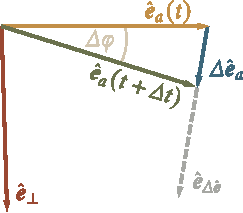
\includegraphics[scale=0.95]{figures/ch_01/fig_1_19.pdf}
		\caption[]{}
		\label{fig:1_19}
	\end{center}
\end{figure}

Đạo hàm của $\vecuni{a}$ theo $t$, theo định nghĩa, bằng
\begin{equation*}
\diff{\vecuni{a}}{t} = \lim_{\Delta t\to 0} \frac{\Delta\vecuni{a}}{\Delta t} = \lim_{\Delta t\to 0} \frac{\Delta\varphi}{\Delta t}\vecuni{\Delta\vec{e}} = \diff{\varphi}{t}\vecuni{\perp}.
\end{equation*}

\noindent
Như vậy,
\begin{equation}\label{eq:1_56}
\dot{\hat{\vec{e}}}_{a} = \dot{\varphi}\vecuni{\perp}.
\end{equation}

\noindent
Đại lượng $\dot{\varphi}=\diffin{\varphi}{t}$ là vận tốc góc quay của vector $\vec{a}$ (xem Sec.~\ref{sec:1_5}). Chuẩn $\vecuni{\perp}$ nằm trong mặt phẳng mà tại đó vector $\vec{a}$ bị quay tại thời điểm đã cho, hơn nữa hướng về phía mà sự quay xảy ra.

\section{Vận tốc}\label{sec:1_3}

Khi chuyển động, chất điểm vẽ một đường nào đó. Đường này được gọi là \textbf{quỹ đạo}\footnote{Ta hãy chú ý rằng khái niệm quỹ đạo chỉ được áp dụng cho hạt ``cổ điển'' mà tại mỗi thời điểm có thể gán cho nó các giá trị chính xác của tọa độ và xung lượng (tức là vận tốc). Theo cơ học lượng tử các hạt có thực có thể được đặc trưng bằng tọa độ và xung lượng chỉ với một độ chính xác nào đó. Giới hạn của độ chính xác này được xác định bằng hệ thức bất định Heisenberg: $\Delta x\Delta p\gtrsim\hbar$. Ở đây $\Delta x$ là độ bất định của tọa độ, $\Delta p$ là độ bất định của xung lượng của hạt, $\hbar$ là hằng số Planck có giá trị bằng $\hbar = h/2\pi = \SI{1.05e-34}{\joule\second}$. Dấu $\gtrsim$ nghĩa là ``lỡn hơn đại lượng vào cỡ''. Nếu thay xung lượng bằng tích khối lượng với vận tốc, thì có thể viết $\Delta x\Delta v\gtrsim\hbar/m$. Từ hệ thức này rõ ràng là khối lượng của hạt càng nhỏ thì tọa độ và vận tốc của nó càng kém được xác định và do đó khái niệm quỹ đạo càng ít được áp dụng. Đối với các vật vĩ mô (tức là các vật được tạo bởi một số rất lớn các phân tử) các độ bất định của tọa độ và vận tốc không vượt quá độ chính xác có thể đạt được trong thực tế khi đo các đại lượng này, do đó khái niệm quỹ đạo có thể áp dụng được cho các vật như thế một cách vô điều kiện. Đối với các hạt vi mô (các electron, proton, neutron, các nguyên tử và phân tử riêng lẻ) tùy thuộc vào các điều kiện trong đó chuyển động xảy ra, khái niệm quỹ đạo hoặc hoàn toàn không áp dụng được hoặc có thể áp dụng được với độ chính xác hạn chế. Chẳng hạn, sự chuyển động của các electron trong ống tia điện tử có thể được coi một cách gần đúng như chuyển động xảy ra theo các quỹ đạo nào đó.}.Tùy theo dạng của quỹ đạo người ta phân biệt chuyển động thẳng, chuyển động tròn, chuyển động cong, v.v...

\begin{figure}[!htb]
	\begin{minipage}[t]{0.5\linewidth}
		\begin{center}
			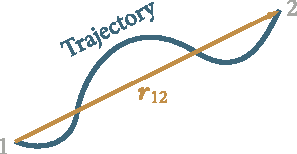
\includegraphics[scale=0.95]{figures/ch_01/fig_1_20.pdf}
			\caption[]{}
			\label{fig:1_20}
		\end{center}
	\end{minipage}
	\hfill{ }%\hspace{-0.1cm}
	\begin{minipage}[t]{0.5\linewidth}
		\begin{center}
			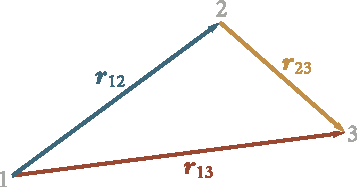
\includegraphics[scale=0.95]{figures/ch_01/fig_1_21.pdf}
			\caption[]{}
			\label{fig:1_21}
		\end{center}
	\end{minipage}
\end{figure}

Giả thử một chất điểm (Sau này để cho gọn ta sẽ gọi nó là một hạt) dịch chuyển dọc theo một quỹ đạo nào đó từ điểm $1$ đến điểm $2$ (\fig{1_20}). Khoảng cách giữa điểm $1$ và $2$ tính dọc theo quỹ đạo được gọi là quãng đường mà hạt đi qua. Ta ký hiệu nó bằng chữ $s$.

Đoạn thẳng vẽ từ điểm $1$ và $2$ được gọi là độ dời của hạt. Ta hãy ký hiệu nó bằng $\vec{r}_{12}$. Ta hãy giả sử rằng hạt thực hiện hai sự dịch chuyển nối tiếp nhau: $\vec{r}_{12}$ và $\vec{r}_{23}$ (\fig{1_21}). Gọi một cách tự nhiên độ dời $\vec{r}_{13}$ mà nó dẫn tới kết quả như hai sự dịch chuyển đầu tiên xảy ra cùng với nhau, là tổng của các độ dời này. Như vậy, các độ dời đều được đặc trưng bằng trị số và hướng và ngoài ra, đều cộng được theo quy tắc hình bình hành. Từ đó suy ra rằng độ dời là một vector.

Trong đời sống hàng ngày người ta hiểu vận tốc là quãng đường vật đi được trong một đơn vị thời gian. Nếu trong những khoảng thời gian bằng nhau và nhỏ tùy ý hạt đi qua những quãng đường như nhau, thì người ta gọi chuyển động của hạt là \textbf{chuyển động đều} . Trong trường hợp này, vận tốc của hạt tại mỗi thời điểm có thể tính bằng cách hcia quãng đường $s$ cho thời gian $t$.

Trong vật lý, người ta hiểu vận tốc là một đại lượng vector đặc trưng không chỉ cho độ nhanh của sự chuyển dời của hạt theo quỹ đạo mà cả cho hướng trong đó hạt chuyển động tại mỗi thời điểm. Ta hãy chia quỹ đạo thành các phần vô cùng nhỏ có độ dài $\mathrm{d}s$. Ta so sánh độ dời vô cùng nhỏ $\mathrm{d}r$ với mỗi phần đó (\fig{1_22}). Chia độ dời này cho khoảng thời gian tương ứng $\mathrm{d}t$, ta được vận tốc tức thời tại điểm đã cho của quỹ đạo:
\begin{equation}\label{eq:1_57}
\vec{v} = \diff{\vec{r}}{t} = \dot{\vec{r}}.
\end{equation}

\noindent
Như vậy vận tốc là đạo hàm của bán kính vector của hạt theo thời gian. Độ dời $\mathrm{d}r$ trùng với yếu tố quỹ đạo vô cùng nhỏ. Do đó vector $\vec{v}$ hướng theo tiếp tuyến của quỹ đạo (xem \fig{1_22}).

\begin{figure}[!htb]
	\begin{minipage}[t]{0.5\linewidth}
		\begin{center}
			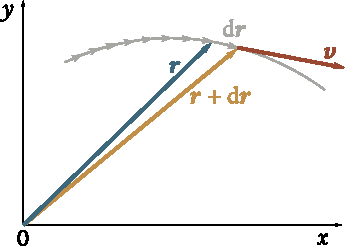
\includegraphics[scale=0.90]{figures/ch_01/fig_1_22.pdf}
			\caption[]{}
			\label{fig:1_22}
		\end{center}
	\end{minipage}
	\hfill{ }%\hspace{-0.1cm}
	\begin{minipage}[t]{0.5\linewidth}
		\begin{center}
			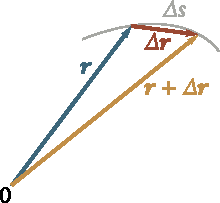
\includegraphics[scale=0.92]{figures/ch_01/fig_1_23.pdf}
			\caption[]{}
			\label{fig:1_23}
		\end{center}
	\end{minipage}
\end{figure}

Nếu lý luận một cách chặt chẽ hơn để có được công thức \eqref{eq:1_57} thì cần phải làm như sau. Bằng cách cố định một thời điểm $t$ nào đó, ta hãy nghiên cứu số gia $\Delta\vec{r}$ của bán kính vector trong khoảng thời gian nhỏ $\Delta t$\footnote{Ký hiệu $\Delta$ (delta) được dùng trong hai trường hợp: (a) để ký hiệu cho số gia của một đại lượng nào đó. Trong trường hợp đang xét, $\Delta\vec{r}$ là số gia của bán kính vector $\vec{r}$ trong thời gian $\Delta t$; (b) để ký hiệu cho một phần của một đại lượng nào đó. Chẳng hạn, $\Delta t$ là một phần của toàn bộ thời gian $t$ trong đó chuyển động xảy ra, $\Delta s$ là một phần của toàn bộ quãng đường $s$ mà hạt đi qua.} tiếp sau $t$ (\fig{1_23}). Tỷ số $\Delta\vec{r}/\Delta t$ cho giá trị trung bình của vận tốc trong khoảng thời gian $\Delta t$. Nếu lấy tất cả các khoảng $\Delta t$ nhỏ thì tỷ số $\Delta\vec{r}/\Delta t$ tại giới hạn cho ta giá trị của vận tốc $\vec{v}$ tại thời điểm $t$:
\begin{equation}\label{eq:1_58}
\vec{v} = \lim_{\Delta t\to 0} \frac{\Delta\vec{r}}{\Delta t} = \diff{\vec{r}}{t}.
\end{equation}

\noindent
Ta đi tới công thức\eqref{eq:1_57}.

Ta hãy tìm module của biểu thức \eqref{eq:1_58}, tức là module của vận tốc $\vec{v}$:
\begin{equation}\label{eq:1_59}
v = |\vec{v}| = \left|\lim_{\Delta t\to 0} \frac{\Delta\vec{r}}{\Delta t}\right| = \lim_{\Delta t\to 0} \frac{|\Delta\vec{r}|}{\Delta t}.
\end{equation}

\noindent
Trong công thức này không được viết $\Delta r$ thay cho $|\Delta\vec{r}|$. Vector $\Delta\vec{r}$ thực chất là hiệu của hai vector ($\vec{r}$ tại thời điểm $t+\Delta t$ trừ $\vec{r}$ tại thời điểm $t$). Do đó có thể viết module của nó bằng các vạch thẳng đứng [xem \eqn{1_2}]. Ký hiệu $|\Delta\vec{r}|$ có nghĩa là module của số gia của vector $\vec{r}$, trong khi mà $\Delta r$ là số gia của module của vector $\vec{r}$: $\Delta|\vec{r}|$. Cả hai đại lượng này nói chung không bằng nhau:
\begin{equation*}
|\Delta\vec{r}| \neq \Delta|\vec{r}| = \Delta r.
\end{equation*}

\noindent
Có thể thấy rõ điều này ở ví dụ sau. Giả sử vector $\vec{r}$ nhận số gia $\Delta\vec{r}$ sao cho module của nó không thay đổi: $|\vec{r}+\Delta\vec{r}|=|\vec{r}|$ (\fig{1_24}). Khi đó số gia của module của vector bằng không ($\Delta|\vec{r}| = \Delta r = 0$). Đồng thời module của số gia của vector $\vec{r}$, tức là $\Delta|\vec{r}|$, là khác không (nó bằng độ dài của đoạn $2-3$). Thật là đối với một vector $\vec{a}$ bất kỳ: trong trường hợp tổng quát $\Delta|\vec{a}|\neq\Delta|a|$.

\begin{figure}[!htb]
	\begin{center}
		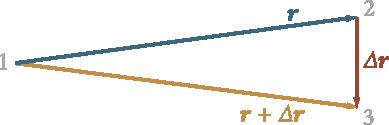
\includegraphics[scale=0.9]{figures/ch_01/fig_1_24.pdf}
		\caption[]{}
		\label{fig:1_24}
	\end{center}
\end{figure}

Từ \fig{1_23} rõ ràng là nói chung quãng đường $\Delta s$ về độ lớn khác với module của độ dời $|\Delta\vec{r}|$. Tuy nhiên nếu lấy đoạn đường $\Delta s$ là độ dời $\Delta\vec{r}$, tương ứng với tất cả khoảng thời gian $\Delta t$ nhỏ thì sự khác nhau giữa $\Delta s$ và $|\Delta\vec{r}|$ sẽ giảm và tỉ số của chúng tại giới hạn trở nên bằng đơn vị:
\begin{equation*}
\lim_{\Delta t\to 0} \frac{\Delta s}{|\Delta\vec{r}|} = 1.
\end{equation*}

\noindent
Trên cơ sở này, có thể thay thế $|\Delta\vec{r}|$ bằng $\Delta s$ trong công thức \eqref{eq:1_59}, kết quả là ta được biểu thức
\begin{equation}\label{eq:1_60}
v = \lim_{\Delta t\to 0} \frac{\Delta s}{\Delta t} = \diff{s}{t}.
\end{equation}

\noindent
Như vậy, module của vận tốc bằng đạo hàm của quãng đường theo thời gian.

Rõ ràng rằng, trong đời sống hàng ngày, đại lượng được gọi là vận tốc thật ralaf module của vận tốc $\vec{v}$. Trong chuyển động đều, module của vận tốc sẽ không đổi ($v=\text{constant}$), trong khi hướng của vector $\vec{v}$ biến đổi một cách tùy ý (trong trường hợp riêng có thể không đổi).

Theo công thức \eqn{1_57} độ dời nguyên tố của hạt bằng
\begin{equation}\label{eq:1_61}
\mathrm{d}\vec{r} = \vec{v}\,\mathrm{d}{t}.
\end{equation}

\noindent
Đôi khi để trực quan, ta ký hiệu độ dời nguyên tố bằng ký hiệu $\mathrm{d}\vec{s}$, nghĩa là viết \eqn{1_61} dưới dạng
\begin{equation}\label{eq:1_62}
\mathrm{d}\vec{s} = \vec{v}\,\mathrm{d}{t}.
\end{equation}

Có thể biểu diễn vector vận tốc cũng như mọi vector khác dưới dạng
\begin{equation}\label{eq:1_63}
\vec{v} = v_x\vecuni{x} + v_y\vecuni{y} + v_z\vecuni{z}
\end{equation}

\noindent
trong đó $v_x, v_y, v_z$ là các hình chiếu của vector $\vec{v}$ lên các trục tọa độ. Ngoài ra, the vector $\dot{\vec{r}}$ bằng $\vec{v}$ theo \eqn{1_43} có dạng như sau:
%\vspace{-12pt}
\begin{equation}\label{eq:1_64}
\dot{\vec{r}} = \dot{x}\vecuni{x} + \dot{y}\vecuni{y} + \dot{z}\vecuni{z}
\end{equation}

\noindent
So sánh các biểu thức \eqref{eq:1_63} và \eqref{eq:1_64} suy ra rằng
\begin{equation}\label{eq:1_65}
v_x = \dot{x},\quad v_y = \dot{y},\quad v_z = \dot{z}.
\end{equation}

\noindent
Do đó, hình chiếu của vector vận tốc lên trục tọa độ bằng đạo hàm theo thời gian của tọa độ tương ứng của hạt chuyển động. Nếu chú ý tới \eqref{eq:1_10} ta có công thức:
\begin{equation}\label{eq:1_66}
v = \sqrt{\dot{x}^2 + \dot{y}^2 + \dot{z}^2}.
\end{equation}

Có thể biểu diễn vector vận tốc dưới dạng $\vec{v}=v\vecuni{v}$, trong đó $v$ là module của vận tốc, còn $\vecuni{v}$ là chuẩn của vector $\vec{v}$. Ta hãy đưa vào chuẩn của tiếp tuyến với quỹ đạo là $\hatvec{\tau}$, quy ước hướng nó theo cùng một phía với $\vec{v}$. Khi đó, rõ ràng rằng các chuẩn $\vecuni{v}$ và $\hatvec{\tau}$ trùng nhau, cho nên có thể viết được biểu thức sau:
%\vspace{-12pt}
\begin{equation}\label{eq:1_67}
\vec{v} = v\vecuni{v} = v\hatvec{\tau}.
\end{equation}

Ta còn có một biểu thúc nữa đối với $\vec{v}$. Với mục đích này ta hãy đặt vào \eqn{1_57} bán kính vector dưới dạng $\vec{r}=r\vecuni{r}$. Theo \eqn{1_49}
\begin{equation}\label{eq:1_68}
\vec{v} = \dot{\vec{r}} = \dot{r}\vecuni{r} + r\dot{\hat{\boldsymbol{e}}}_r.
\end{equation}

\noindent
Để đơn giản hãy giới hạn ở trường hợp khi quỹ đạo là một đường cong phẳng, nghĩa là một đường cong mà mọi điểm của nó nằm trên một mặt phẳng. Ta hãy dùng mặt phẳng này làm mặt phẳng $x, y$. Trong \eqn{1_68}, vector $\vec{v}$ được biểu diễn dưới dạng tổng của hai thành phần (\fig{1_25}). Thành phần thứ nhất mà ta ký hiệu là $\vec{v}_r$ bằng
\begin{equation}\label{eq:1_69}
\vec{v}_r = \dot{r}\vecuni{r}.
\end{equation}

\begin{figure}[!htb]
	\begin{center}
		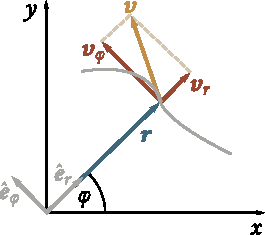
\includegraphics[scale=1]{figures/ch_01/fig_1_25.pdf}
		\caption[]{}
		\label{fig:1_25}
	\end{center}
\end{figure}


\noindent
Nó hướng dọc theo bán kính vector $\vec{r}$ và đặc trưng cho độ nhanh của sự biến đổi module của $\vec{r}$. Thành phần thú hai mà ta ký hiệu là $\vec{v}_{\varphi}$ bằng
\begin{equation}\label{eq:1_70}
\vec{v}_{\varphi} = r\dot{\hat{\boldsymbol{e}}}_r.
\end{equation}

\noindent
Nó đặc trưng cho độ nhanh của sự biến đổi về hướng của bán kính vector.

Dùng \eqn{1_56} có thể viết là
\begin{equation*}
\dot{\hat{\boldsymbol{e}}}_r = \diff{\varphi}{t}\vecuni{\varphi} = \dot{\varphi}\vecuni{\varphi}
\end{equation*}

\noindent
trong đó $\varphi$ là góc giữa bán kính vector và trục $x$, $\vecuni{\varphi}$ là chuẩn vuông góc với bán kính vector hướng về phía tăng của góc $\varphi$ [trong \eqn{1_56} chuẩn được ký hiệu là $\vecuni{\perp}$]. Thế giá gị này vào \eqn{1_70} ta có:
\begin{equation}\label{eq:1_71}
\vec{v}_{\varphi} = r\dot{\varphi}\vecuni{\varphi}.
\end{equation}

\noindent
Ta đưa vào các ký hiệu $\vec{v}_{\varphi}$ và $\vecuni{\varphi}$ để nhấn mạnh rằng thành phần $\vec{v}_{\varphi}$ và chuẩn tương ứng liên hệ với sự biến đổi của góc $\varphi$.

Rõ ràng rằng, các vector $\vec{v}_r$ và $\vec{v}_{\varphi}$ vuông góc với nhau. Do đó
\begin{equation}\label{eq:1_72}
v = \sqrt{v_r^2 + v_{\varphi}^2} = \sqrt{\dot{r}^2 + r^2\dot{\varphi}^2}.
\end{equation}

Ta hãy xét bài toán là khi biết độ lớn của vận tốc tại mỗi thời điểm, hãy tính quãng đường mà hạt đi qua từ thời điể $t_1$ đến thời điểm $t_2$. Ta chia khoảng thời gian $t_2-t_1$ thành $N$ khoảng nhỏ, không nhất thiết phải bằng nhau: $\Delta t_1$, $\Delta t_2$, \ldots, $\Delta t_N$. Có thể biểu diễn toàn bộ quãng đường $s$ mà hạt đi được như là tổng các quãng đường $\Delta s_1$, $\Delta s_2$, \ldots, $\Delta s_N$ mà hạt đi được trong những khoảng thời gian $\Delta t$ tương ứng:
\begin{equation*}
s = \Delta s_1 + \Delta s_2 + \ldots + \Delta s_N = \sum_{i=1}^{N} \Delta s_i.
\end{equation*}

\noindent
Theo \eqn{1_60}, mỗi số hạng có thể biểu diễn gần đúng dưới dạng
\begin{equation*}
\Delta s_i \approx v_i \Delta t_i
\end{equation*}

\noindent
trong đó $\Delta t_i$ là khoảng thời gian mà hạt đi được một quãng đường $\Delta s_i$, còn $v_i$ là giá trị của vạn tốc trong khoảng thời gian $\Delta t_i$. Do đó
\begin{equation}\label{eq:1_73}
s \approx \sum_{i=1}^{N} v_i \Delta t_i.
\end{equation}

\noindent
Đằng thức trên càng chính xác nếu khoảng thời gian $\Delta t_i$ càng nhỏ. Tại giới hạn khi tất cả các khoảng $\Delta t_i$ tiến tới không (số lượng các khoảng $\Delta t_i$ khi đó tăng vô hạn) thì đẳng thức gần đúng trở thành đẳng thức đúng:
\begin{equation*}
s = \lim_{\Delta t_i\to 0} \sum_{i=1}^{N} v_i \Delta t_i.
\end{equation*}

Biểu thức thu được là một tích phân xác định của hàm $v(t)$ lấy trong phạm vi từ $t_1$ đến $t_2$. Như vậy, quãng đường mà hạt đi được trong khoảng thời gian từ $t_1$ đến $t_2$ bằng
\begin{equation}\label{eq:1_74}
s = \int_{t_1}^{t_2} v(t)\,\mathrm{d}t.
\end{equation}

\noindent
Ta hãy nhấn mạnh rằng ở đây nói về module của vận tốc. Nếu lấy tích phân của chính vận tốc $\vec{v}(t)$ thì người ta thu được vector độ dời của hạt tử điểm mà hạt nằm ở thời điểm $t_1$ tới điểm mà hạt nằm ở thời điểm $t_2$:
\begin{equation}\label{eq:1_75}
\int_{t_1}^{t_2} v(t)\,\mathrm{d}t = \int_{t_1}^{t_2} \mathrm{d}\vec{r} = \vec{r}_{12}
\end{equation}

\noindent
[xem \eqn{1_61}].

Nếu vẽ đồ thị biểu diễn sự phụ thuộc của $v$ theo $t$ (\fig{1_26}) thì có thể biểu diễn quãng đường đi được như diện tích của hình được giwois hạn bởi đường cong $v(t)$ và các đường thẳng $t = t_1$ và $t = t_2$. Thật vậy, tích $v_i\Delta t_i$ nvề trị số bằng diện tích của dải thứ $i$. Tổng \eqn{1_73} bằng diện tích được giới hạn về phía trên bởi đường gấp khúc tạo bởi các mép trên của tất cả các dải tương tự. Khi tất cả $\Delta t_i$ tiến tới không độ rộng của các dải giảm (đồng thời số các dải tăng) và đường gấp khúc tại giới hạn trùng với đường cong $v = v(t)$. Như vậy quãng đường đi được trong thời điểm $t_1$ đến thời điểm $t_2$ về trị số bằng diện tích giới hạn bởi đồ thị của hàm $v = v(t)$, trục thời gian $t$ và các đường thẳng $t= t_1$ và $t = t_2$.

\begin{figure}[!htb]
	\begin{center}
		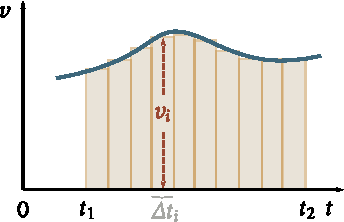
\includegraphics[scale=1]{figures/ch_01/fig_1_26.pdf}
		\caption[]{}
		\label{fig:1_26}
	\end{center}
\end{figure}

Ta hãy chú ý rằng giá trị trung bình của module của vận tốc trong khoảng thời gian từ $t_1$ đến  $t_2$ theo định nghĩa bằng
\begin{equation*}
\average{v} = \frac{s}{t_2-t_1}.
\end{equation*}

\noindent
(The symbol $\langle\rangle$ embracing the $v$ indicates an average.) Thay thế biểu thức \eqref{eq:1_74} đối với $s$ vào đây ta có:
\begin{equation}\label{eq:1_76}
\average{v} = \frac{1}{t_2-t_1}\,\int_{t_1}^{t_2}v(t)\,\mathrm{d}t.
\end{equation}

\noindent
Người ta tính các giá trị trung bình của các hàm vô hướng hay các hàm vector bất kỳ cũng tương tự như vật. Chẳng hạn, giá trị trung bình của vận tốc bằng
\begin{equation}\label{eq:1_77}
\average{\vec{v}} = \frac{1}{t_2-t_1}\,\int_{t_1}^{t_2}\vec{v}(t)\,\mathrm{d}t = \frac{\vec{r}_{12}}{t_2-t_1}.
\end{equation}

\noindent
[xem \eqn{1_75}]. Các giá trị trung bình của hàm $y(x)$ trong khoảng từ $x_1$ đến $x_2$ được xác định bằng biểu thức
\begin{equation}\label{eq:1_78}
\average{y} = \frac{1}{t_2-t_1}\,\int_{x_1}^{x_2}y(t)\,\mathrm{d}x.
\end{equation}

\section{Gia tốc}\label{sec:1_4}

Vận tốc $\vec{v}$ của hạt có thể biến đổi theo thời gian cả về độ lớn lẫn hướng. Độ nhanh của sự thay đổi của vector $\vec{v}$ cũng như độ nhanh của sự thay đổi của một hàm bất kỳ của thời gian được định nghĩa bằng đạo hàm của vector $\vec{v}$ theo $t$. Nếu ký hiệu đạo hàm này bằng chữ $\vec{a}$ thì ta có:
\begin{equation}\label{eq:1_79}
\vec{a} = \lim_{\Delta t\to 0}\frac{\Delta\vec{v}}{\Delta t} = \diff{\vec{v}}{t} = \dot{\vec{v}}.
\end{equation}

\noindent
Đại lượng xác định bằng công thức \eqref{eq:1_79} được gọi là \textbf{gia tốc} của hạt.

Ta chú ý rằng vector $\vec{v}$ có vai tròn như thế nào đối với bán kính vector $\vec{r}$ thì gia tốc $\vec{a}$ có vai trò như thế đối với $\vec{v}$.

Các vector bằng nhau có hình chiếu lên các trục tọa độ như nhau. Do đó, chẳng hạn
\begin{equation*}
a_x = \left(\diff{\vec{v}}{t}\right)_{\text{pr. }\vec{x}} = \diff{v_x}{t} = \dot{v}_x
\end{equation*}

\noindent
[xem Eqs.~\eqref{eq:1_40}]. Đồng thời, theo Eqs.~\eqref{eq:1_65}, we have $v_x=\dot{x}=\diffin{x}{t}$. Do đó
\begin{equation*}
\diff{v_x}{t} = \frac{\mathrm{d}}{\mathrm{d}t} \left(\diff{x}{t}\right) = \diffsec{x}{t} = \ddot{x}.
\end{equation*}

\noindent
Ta đã có hình chiếu của vector gia tốc lên trục $x$ bằng đạo hàm bậc hai của tọa độ x theo thời gian: $a_x=\ddot{x}$. Một cách tương tự, người ta cũng có được các biểu thức đối với hình chiếu của gia tốc lên các trục $y$ và $z$. Như vậy,
\begin{equation}\label{eq:1_80}
a_x=\ddot{x},\quad a_y=\ddot{y},\quad a_z=\ddot{z}.
\end{equation}

Ta hãy thay thế \eqn{1_67} đối với $\vec{v}$  vào công thức \eqref{eq:1_79}:
\begin{equation}\label{eq:1_81}
\vec{a} = \diff{(v\hatvec{\tau})}{t}.
\end{equation}

\noindent
Ta nhớ rằng $\hatvec{\tau}$ là chuẩn của tiếp tuyến với quỹ đạo, hướng về cùng phía với $\vec{v}$. Theo \eqn{1_49},
\begin{equation}\label{eq:1_82}
\vec{a} = \dot{v}\hatvec{\tau} + v\dot{\hatvec{\tau}}.
\end{equation}

\noindent
Do đó có thể biểu diễn vector $\vec{a}$ dưới dạng tổng của hai thành phần. Một thành phần cùng phương với $\hatvec{\tau}$, tức là hướng theo tiếp tuyến với quỹ đạo, và do đó được ký hiệu là $\vec{a}_{\hatvec{\tau}}$ và được gọi là \textbf{gia tốc tiếp tuyến}. Nó bằng
\begin{equation}\label{eq:1_83}
\vec{a}_{\hatvec{\tau}} = \dot{v}\hatvec{\tau}.
\end{equation}

\noindent
Thành phần thứ hai bằng $v\dot{\hatvec{\tau}}$, như ta sẽ chứng tỏ ở dưới đây, hướng theo pháp tuyến với quỹ đạo và do đó được ký hiệu là $\vec{a}_{\hatvec{n}}$ và được gọi là \textbf{gia tốc pháp tuyến}. Như vậy,
\begin{equation}\label{eq:1_84}
\vec{a}_{\hatvec{n}} = v\dot{\hatvec{\tau}}.
\end{equation}

Ta hãy nghiên cứu các tính chất của cả hai thành phần, để đơn giản chỉ bó hẹp ở trường hợp khi quỹ đạo là một đường cong phẳng.

Module của gia tốc tiếp tuyến \eqref{eq:1_83} bằng
\begin{equation}\label{eq:1_85}
\vec{a}_{\hatvec{\tau}} = |\dot{v}|.
\end{equation}

\noindent
Nếu $\dot{v}>0$ (vận tốc tăng về độ lớn), thì vector $\vec{a}_{\hatvec{\tau}}$ có cùng hướng với $\hatvec{\tau}$ (tức là có cùng hướng với $\vec{v}$). Nếu $\dot{v}<0$ (vận tốc giảm theo thời gian), thì các vector $\vec{v}$ và $\vec{a}_{\hatvec{\tau}}$ hướng theo các chiều ngược nhau. Trong chuyển đông đều $\dot{v}=0$, và do đó không có gia tốc tiếp tuyến.

Để làm rõ các tính chất của gia tốc pháp tuyển [\eqn{1_84}] cần phải xác minh xem $\dot{\hatvec{\tau}}$, tức là độ nhanh của sự thay đổi theo thời gian của hướng tiếp tuyến với quỹ đạo, sẽ được xác định bằng cái gì. Dễ dàng hiểu được rằng độ nhanh này sẽ càng lớn khi độ cong của quỹ đạo càng lớn và khi hạt dịch chuyển càng nhanh theo quỹ đạo.

Mức độ cong của đường cong phẳng được đặc trưng bằng độ cong $C$, mà nó được định nghĩa bằng biểu thức
\begin{equation}\label{eq:1_86}
C = \lim_{\Delta t\to 0} \frac{\Delta\varphi}{\Delta s} = \diff{\varphi}{s}
\end{equation}

\noindent
trong đó $\Delta\varphi$ là góc giữa các tiếp tuyến với đường cong tại các điểm cách nhau một khoảng $\Delta s$ (\fig{1_27}). Như vậy độ cong xác định vận tốc quay của tiếp tuyến khi dịch chuyển dọc theo đường cong.

\begin{figure}[!htb]
	\begin{center}
		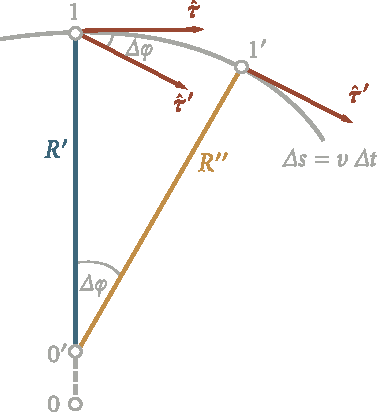
\includegraphics[scale=1]{figures/ch_01/fig_1_27.pdf}
		\caption[]{}
		\label{fig:1_27}
	\end{center}
\end{figure}


Đại lượng nghịch đảo của độ cong $C$ được gọi là \textbf{bán kính cong} của đường cong tại điểm đã cho và được ký hiệu bằng chữ $R$:
The degree of bending of a plane curve is characterized by its curvature $C$ determined by the expression
\begin{equation}\label{eq:1_87}
R = \frac{1}{C} = \lim_{\Delta\varphi\to 0} \frac{\Delta s}{\Delta\varphi} = \diff{s}{\varphi}.
\end{equation}

\noindent
Bán kính cong là bán kính của một đường tròn mà nó nhập vào đường cong tại một phần vô cùng nhỏ của nó ở điểm đã cho. Tâm của đường tròn này được gọi là tâm cong đối với điểm đã cho của đường cong.

Bán kính cong và tâm cong tại điểm $1$ (xem \fig{1_27}) Có thể được xác định bằng cách sau. Ta hãy lấy điểm $1'$ không xa $1$. Vẽ các tiếp tuyến $\hatvec{\tau}$ và $\hatvec{\tau}'$ tại các điểm này. Các đường thẳng vuông góc với các tiếp tuyến cắt nhau tại một điểm $0'$. Ta chú ý rằng đối với một đường cong không phải là đường tròn, các khoảng cách $R'$ và $R''$ sẽ khác nhau rất ít. Nếu dịch điểm $1'$ lại gần điểm $1$, thì giao điểm $0'$ của các đường vuông góc sẽ dịch chuyển dọc theo đường thẳng $R'$ và tại giới hạn nó nằm tại một điểm $0$ nào đó. Chính điểm này là tâm cong đối với điểm $1$. Các khoảng cách $R'$ và $R"$ sẽ tiến đến một giới hạn chung $R$ bằng bán kính cong. Thực vậy, nếu các điểm $1$ và $1'$ ở gần nhau thì có thể viết là $\Delta\varphi\approx\Delta s/R'$ or $R' \approx \Delta s/\Delta\varphi$. Tại giới hạn khi $\Delta\varphi\to 0$ thì đẳng thức gần đúng này chuyển về đẳng thức thực sự $R=\diffin{s}{\varphi}$, trùng với định nghĩa của bán kính cong [xem \eqn{1_87}].

Ta hãy trở lại cách tính $\vec{a}_{\hatvec{n}}$ [xem \eqn{1_84}]. Theo \eqn{1_56},
\begin{equation}\label{eq:1_88}
\dot{\hatvec{\tau}} = \diff{\varphi}{t}\hatvec{n}
\end{equation}

\noindent
trong đó $\hatvec{n}$ là chuẩn của pháp tuyến với quỹ đạo, hướng về phía mà khi hạt chuyển động theo quỹ đạo thì vector $\hatvec{\tau}$ quay về phía đó [trong \eqn{1_56} chuẩn tương tự đã được ký hiệu bằng $\vecuni{\perp}$]. Có thể liên kết đại lượng $\diffin{\varphi}{t}$ với bán kính cong của quỹ đạo và vận tốc $\vec{v}$ của hạt. Từ \fig{1_27} suy ra rằng
\begin{equation*}
\Delta\varphi\approx \frac{\Delta s}{R'} = \frac{v'\,\Delta t}{R'}
\end{equation*}

\noindent
trong đó $\Delta\varphi$ là góc quay của vector $\hatvec{\tau}$ trong khoảng thời gian $\Delta t$ (trùng với góc giữa các đường vuông góc $R'$ và $R''$), $v'$ là vận tốc trung bình trên quãng đường $\Delta s$. Từ đây
\begin{equation*}
\frac{\Delta\varphi}{\Delta s} \approx \frac{v'}{R'}.
\end{equation*}

\noindent
Tại giới hạn khi $\Delta t\to 0$ không đẳng thức gần đúng trở thành đẳng thức thực sự, vạn tốc trung bình $v'$ trở thành vận tốc tức thời $v$ tại thời điểm $1$, $R'$ trở thành bán kính cong $R$. Kết quả là ta có đẳng thức
\begin{equation}\label{eq:1_89}
\diff{\varphi}{t} = \frac{v}{R} = vC
\end{equation}

\noindent
($C$ là độ cong).Do đó độ nhanh của sự quay vector vận tốc, như ta đã giả thử, sẽ tỷ lệ với độ cong của quỹ đạo và vận tốc chuyển dời của hạt theo quỹ đạo.

Thay \eqn{1_89} vào \eqref{eq:1_88} ta được $\dot{\hatvec{\tau}}=(v/R)\hatvec{n}$. Sau cùng, introducing thay biểu thúc này vào \eqn{1_84}, ta đi tới công thức cuối cùng đối vwois gia tốc pháp tuyến:
%\vspace{-12pt}
\begin{equation}\label{eq:1_90}
\vec{a}_{\hatvec{n}} = \diff{v^2}{R}\hatvec{n}.
\end{equation}

Vậy vector gia tốc khi hạt chuyển động theo đường cong phẳng được xác định bởi biểu thức sau:
\begin{equation}\label{eq:1_91}
\vec{a} = \vec{a}_{\hatvec{\tau}} + \vec{a}_{\hatvec{n}} = \dot{v}\hatvec{\tau} + \frac{v^2}{R}\hatvec{n}.
\end{equation}

\noindent
Module của vector $\vec{a}$ bằng
\begin{equation}\label{eq:1_92}
a = \sqrt{a_{\hatvec{\tau}}^2 + a_{\hatvec{n}}^2} = \sqrt{\dot{v}^2 + \left(\frac{v^2}{R}\right)^2}.
\end{equation}

Trong chuyển động thẳng gia tốc pháp tuyến không có mặt. Ta hãy chú ý rằng $\vec{a}_{\hatvec{n}}$ triệt tiêu tại điểm uốn của quỹ đạo cong (tại điểm IP trên \fig{1_28}). Về cả hai bên của điểm này các vector $\vec{a}_{\hatvec{n}}$ hướng về các phía khác nhau. Vector $\vec{a}_{\hatvec{n}}$ không thể biến đổi nhảy vọt; sự thay đổi hướng ngược lại xảy ra một cách đều đặn với sự triệt tiêu của $\vec{a}_{\hatvec{n}}$ tại điểm uốn. Giả sử hạt chuyển động đều với gia tốc không thay đổi về độ lớn nên $\vec{a}_{\hatvec{\tau}}=0$, cho nên $\vec{a}=\vec{a}_{\hatvec{n}}$. Sự không thay đổi về độ lớn của $\vec{a}_{\hatvec{n}}$ có nghĩa là $v^2/R=\text{constant}$. Từ đó ta kết luận rằng $R=\text{constant}$ ($v=\text{constant}$ do chuyển động đều). Như thế là, hạt chuyển động theo đường cong có độ cong không đổi, tức là theo đường tròn. Vì vậy trong trường hợp mà gia tốc của hạt không đổi về độ lớn và tại mỗi thời điểm được hướng vuông góc với vector vận tốc, thì đường tròn là quỹ đạo của hạt.

\begin{figure}[!htb]
	\begin{center}
		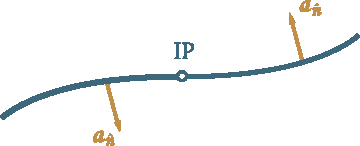
\includegraphics[scale=0.95]{figures/ch_01/fig_1_28.pdf}
		\caption[]{}
		\label{fig:1_28}
	\end{center}
\end{figure}

\section{Động học của chuyển động quay}\label{sec:1_5}

Có thể biểu diễn sự quay một vật một góc $\varphi$ nào đó dưới dạng một đoạn thẳng có độ dài bằng $\varphi$, còn hướng trùng với trục quay. Để chỉ ra phép quay xung quanh trục đã cho được thực hiện theo chiều nào, người ta gắn chiều quay và đoạn thẳng biểu diễn nó bằng \textbf{quy tắc cái đinh ốc thuận}: chiều của đoạn thẳng phải như thế nào để khi nhìn dọc theo nó (\fig{1_29}) ta thấy sự quay được thực hiện theo chiều kim đồng hồ (khi quay đầu đinh ốc thuận theo chiều kim đồng hồ ta làm cho nó dịch chuyển theo chính nó). Trong \ref{sec:1_2} đã chứng tỏ (xem \fig{1_4}) rằng các sự quay những góc hữu hạn được cộng không theo quy tắc hình bình hành và do đó không là những vector. Đối với các sự quay các góc rất nhỏ $\Delta\vec{\varphi}$ thì lại khác. Quãng đường mà một điểm bất kỳ của vật đi được trong sự quay rất nhỏ có thể được coi là quãng đường thẳng (\fig{1_30}). Do đó hai sự quay nhỏ $\Delta\vec{\varphi}_1$ và $\Delta\vec{\varphi}_2$ được thực hiện liên tiếp, như đã thấy trên hình vẽ, gây ra cùng một sự dịch chuyển $\Delta\vec{r}_3=\Delta\vec{r}_1+\Delta\vec{r}_2$ của một điểm bất kỳ của vật như sự quay $\Delta\vec{\varphi}_3$ thu được từ $\Delta\vec{\varphi}_1$ và $\Delta\vec{\varphi}_2$ bằng cách cộng theo quy tắc hình bình hành. Từ đó suy ra rằng có thể coi các sự quay rất nhỏ như các vector (ta ký hiệu các vector này bằng ký hiệu $\Delta\vec{\varphi}$ hoặc $\mathrm{d}\vec{\varphi}$). Hướng của vector quay gắn liền với hướng quay của vật. Do đó $\mathrm{d}\vec{\varphi}$ không là một vector thực mà là một giả vector.

\begin{figure}[!htb]
	\begin{minipage}[t]{0.5\linewidth}
		\begin{center}
			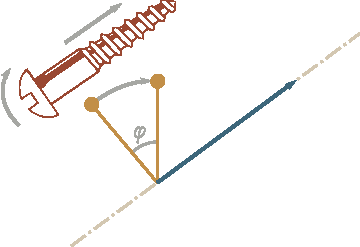
\includegraphics[scale=0.95]{figures/ch_01/fig_1_29.pdf}
			\caption[]{}
			\label{fig:1_29}
		\end{center}
	\end{minipage}
	\hfill{ }%\hspace{-0.1cm}
	\begin{minipage}[t]{0.5\linewidth}
		\begin{center}
			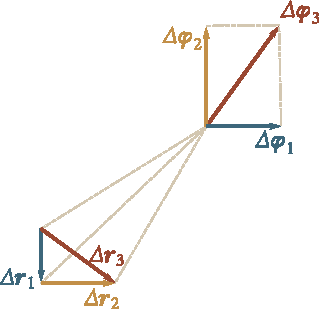
\includegraphics[scale=0.95]{figures/ch_01/fig_1_30.pdf}
			\caption[]{}
			\label{fig:1_30}
		\end{center}
	\end{minipage}
\end{figure}

Đại lượng vector
\begin{equation}\label{eq:1_93}
\vec{\omega} = \lim_{\Delta t\to 0} \frac{\Delta\vec{\varphi}}{\Delta t} = \diff{\vec{\varphi}}{t}
\end{equation}

\noindent
(trong đó $\Delta t$ là thời gian mà sự quay $\Delta\vec{\varphi}$ được thực hiện) được gọi là vận tốc góc của vật\footnote{Vận tốc $\vec{v}$  được khảo sát trong \ref{sec:1_3} đôi khi được gọi là vận tốc dài.}. Vận tốc góc $\vec{\omega}$ hướng dọc theo trục quay của vật theo chiều được xác định bằng quy tắc cái đinh ốc thuận (\fig{1_31}) và là một giả vector. Module của vận tốc góc bằng $\diffin{\varphi}{t}$. Sự quay với vận tốc góc không đổi được gọi là sự quay đều. Nếu sự quay là đều thì $\omega=\varphi t$, trong đó $\varphi$ là góc quay hữu hạn trong thời gian $t$ (so sánh với $v=s/t$). Như vậy trong sự quay đều, $\omega$ chỉ rõ vật quay được góc nào trong một đơn vị thời gian.

\begin{figure}[!htb]
	\begin{minipage}[t]{0.5\linewidth}
		\begin{center}
			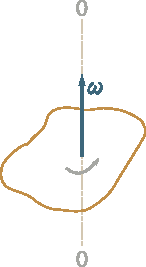
\includegraphics[scale=1]{figures/ch_01/fig_1_31.pdf}
			\caption[]{}
			\label{fig:1_31}
		\end{center}
	\end{minipage}
	\hspace{-0.1cm}
	\begin{minipage}[t]{0.5\linewidth}
		\begin{center}
			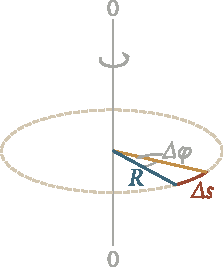
\includegraphics[scale=0.95]{figures/ch_01/fig_1_32.pdf}
			\caption[]{}
			\label{fig:1_32}
		\end{center}
	\end{minipage}
	\vspace{-0.5cm}
\end{figure}

Có thể đặc trưng sự quay đều bằng chu kỳ quay $T$, được hiểu là thời gian trong đó vật quay một vòng, nghĩa là quay một góc $2\pi$. Vì khoảng thời gian $\Delta t=T$ ứng với góc quay $\Delta\varphi=2\pi$, nên
\begin{equation}\label{eq:1_94}
\omega = \frac{2\pi}{T}
\end{equation}

\noindent
từ đó
\begin{equation}\label{eq:1_95}
T = \frac{2\pi}{\omega}.
\end{equation}

Số vòng $\nu$ trong một đơn vị thời gian rõ ràng bằng
\begin{equation}\label{eq:1_96}
\nu = \frac{1}{T} = \frac{\omega}{2\pi}.
\end{equation}

\noindent
Từ \eqn{1_96} suy ra rằng vận tốc góc sẽ bằng $2\pi$ nhân với số vòng trong một đơn vị thời gian:
\begin{equation}\label{eq:1_97}
\omega = 2\pi\nu.
\end{equation}

Có thể giữ nguyên khái niệm chu kỳ quay và số vòng trong một đơn vị thời gian cho cả sự quay không đều bằng cách hiểu giá trị tức thời $T$ là thời gian mà vật có thể thực hiện một vòng nếu nó quay đều với giá trị tức thời đã cho của vận tốc góc, còn $\nu$ được hiểu là số vòng mà vật thực hiện trong một đơn vị thời gian trong những điều kiện tương tự.

Vector $\vec{\omega}$ có thể biến đổi do sự biến đổi của vận tốc quay của vật xung quanh một trục (trong tường hợp này nó biến đổi về độ lớn) cũng như do sự quay của trục quay trong không gian (trong trường hợp này $\vec{\omega}$ biến đổi về hướng). Giả sử trong thời gian $\Delta t$, vector $\vec{\omega}$ nhận số gia $\Delta\vec{\omega}$. Sự biến đổi của vector vận tốc góc theo thời gian được đặc trưng bằng đại lượng
\begin{equation}\label{eq:1_98}
\vec{\alpha} = \lim_{\Delta t\to 0} \frac{\Delta\vec{\omega}}{t} = \diff{\vec{\omega}}{t}
\end{equation}

\noindent
được gọi là \textbf{gia tốc góc}. Gia tốc góc cũng như vận tốc góc là một giả vector.

\begin{figure}[!htb]
	\begin{center}
		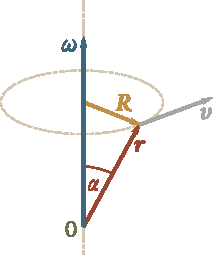
\includegraphics[scale=1]{figures/ch_01/fig_1_33.pdf}
		\caption[]{}
		\label{fig:1_33}
	\end{center}
\end{figure}

Các điểm riêng biệt của một vật quay sẽ có các vận tóc dài $\vec{v}$ khác nhau. Vận tốc của từng điểm biến đổi phương liên tục. Độ lớn $v$ của vận tốc được xác định bằng vận tốc quay $\omega$ của vật và khoảng cách $R$ từ điểm được xét đến trục quay. Giả sử trong khoảng thời gian nhỏ vật quay được một góc $\Delta\varphi$ (\fig{1_32}). Đồng thời điểm ằm cách trục một khoảng $R$ sẽ đi được một quãng đường $\Delta s=R\Delta\varphi$. Vận tốc dài của điểm sẽ bằng
\begin{equation*}
v = \lim_{\Delta t\to 0} \frac{\Delta s}{\Delta t} = \lim_{\Delta t\to 0} R\frac{\Delta\varphi}{\Delta t} = R \lim_{\Delta t\to 0} \frac{\Delta\varphi}{\Delta t} = R\diff{\varphi}{t} = R\omega.
\end{equation*}

\noindent
Như vậy
\begin{equation}\label{eq:1_99}
v = \omega R.
\end{equation}

Công thức \eqref{eq:1_99} liên hệ các module của vận tốc dài và vận tốc góc. Ta hãy tìm biểu thức liên hệ các vector $\vec{v}$ và $\vec{\omega}$. Vị trí của điểm đang xét của vật sẽ được xác định bằng bán kính vector $\vec{r}$ vẽ từ gốc tọa độ $O$ nằm trên trục quay (\fig{1_33}). Từ hình vẽ ta thấy rằng tích vector $\vecprod{\omega}{r}$ trùng về hướng tới vector $\vec{v}$ và có module bằng $\omega r\sin\alpha=\omega R$. Do đó,
\begin{equation}\label{eq:1_100}
\vec{v} = \vecprod{\omega}{r}.
\end{equation}

Module của gia tốc pháp tuyến của các điểm của vật quay bằng $\vec{a}_{\hatvec{n}}=v^2/R$. Thế giá trị $v$ từ \eqn{1_99} vào đây ta có
\begin{equation}\label{eq:1_101}
a_{\hatvec{n}} = \omega^2 R.
\end{equation}

\noindent
Nếu đưa vào vector $\vec{R}$ vuông góc với trục quay, vẽ từ điểm đã cho của vật (xem \fig{1_33}), thì có thể viết \eqn{1_101} dưới dạng vector:
\begin{equation}\label{eq:1_102}
\vec{a}_{\hatvec{n}} = -\omega^2 \vec{R}.
\end{equation}

\noindent
Trong công thức này có dấu trừ bởi vì các vector $\vec{a}_{\hatvec{n}}$ và $\vec{R}$ có các chiều ngược nhau.

Ta hãy giả thử rằng trục quay của vật không quay trong không gian. Theo \eqn{1_85} module của gia tốc tiếp tuyến bằng $|\diffin{v}{t}|$. Sử dụng hệ thức \eqref{eq:1_99} và chú ý đến khoảng cách $R=\text{constant}$ từ điểm đang xét của vật đến trục quay, có thể viết
\begin{equation*}
a_{\hatvec{\tau}} = \left| \lim_{\Delta t\to 0} \frac{\Delta v}{\Delta t} \right| = \left| \lim_{\Delta t\to 0} \frac{\Delta(\omega R)}{\Delta t} \right| = R \left| \lim_{\Delta t\to 0} \frac{\Delta(\omega)}{\Delta t} \right| = R\alpha
\end{equation*}

\noindent
trong $\alpha$ là module của gia tốc góc. Do đó module của gia tốc tiếp tuyến liên hệ với module của gia tốc góc bằng hệ thức:
\begin{equation}\label{eq:1_103}
a_{\hatvec{\tau}} = \alpha R.
\end{equation}

Như vậy gia tốc pháp tuyến và tiếp tuyến tăng tuyến tính với sự tăng của khoảng cách từ điểm tới trục quay.
